\documentclass{scrreprt}
\usepackage[left=2cm,right=2cm,top=2cm,bottom=2cm,includeheadfoot]{geometry}
\usepackage[usenames]{color}
\usepackage{tikz}
\usetikzlibrary{mindmap,trees,decorations,decorations.pathreplacing,decorations.pathmorphing,calc}
\usepackage{pstricks}

\usepackage{hyperref}
\usepackage{listings}
\lstset{breaklines=true,basicstyle=\ttfamily}

\begin{document}
\tableofcontents
%\part{Wintersemester 2008/2009}
%\chapter{Physik}
\section{11.12.2008}
\subsection{11.12.2008-IMG-phys-1}
\begin{tikzpicture}
	\draw[thick] (0,0) node [left] {$G$} -- (2,0);
	\draw[thick] (0,0) circle (0.07);
	\draw[thick] (2,1) -- (2,-1);

	\draw[thick] (3,1) -- (3,-1);

	\draw[thick] (3,1) -- (4,1) -- (4,3) node [right] {$D$};
	\draw[thick] (4,3) circle (0.07);

	\draw[thick] (3,-1) -- (4,-1) -- (4,-3) node [right] {$S$};
	\draw[thick] (4,-3) circle (0.07);

	\draw[thick] (3,0) -- (5,0) node [right] {$B$};
	\draw[thick] (5,0) circle (0.07);
\end{tikzpicture}
\begin{lstlisting}[frame=single]
\begin{tikzpicture}
	\draw[thick] (0,0) node [left] {$G$} -- (2,0);
	\draw[thick] (0,0) circle (0.07);
	\draw[thick] (2,1) -- (2,-1);

	\draw[thick] (3,1) -- (3,-1);

	\draw[thick] (3,1) -- (4,1) -- (4,3) node [right] {$D$};
	\draw[thick] (4,3) circle (0.07);

	\draw[thick] (3,-1) -- (4,-1) -- (4,-3) node [right] {$S$};
	\draw[thick] (4,-3) circle (0.07);

	\draw[thick] (3,0) -- (5,0) node [right] {$B$};
	\draw[thick] (5,0) circle (0.07);
\end{tikzpicture}
\end{lstlisting}

\subsection{11.12.2008-IMG-phys-3}
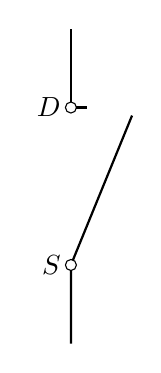
\begin{tikzpicture}
	\draw[thick] (0,0) -- (0,1) node [left] {$S$} -- (75:3);
	\draw[thick] (0.2,3) -- (0,3) node [left] {$D$} -- (0,4);

	\draw[fill=white] (0,1) circle (0.07);
	\draw[fill=white] (0,3) circle (0.07);
\end{tikzpicture}
\begin{lstlisting}[frame=single]
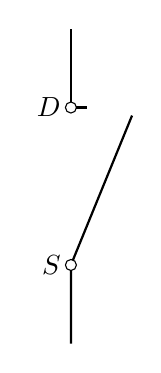
\begin{tikzpicture}
	\draw[thick] (0,0) -- (0,1) node [left] {$S$} -- (75:3);
	\draw[thick] (0.2,3) -- (0,3) node [left] {$D$} -- (0,4);

	\draw[fill=white] (0,1) circle (0.07);
	\draw[fill=white] (0,3) circle (0.07);
\end{tikzpicture}
\end{lstlisting}

\subsection{11.12.2008-IMG-phys-4}
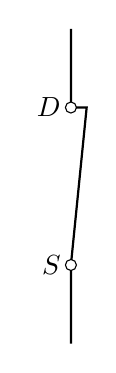
\begin{tikzpicture}
	\draw[thick] (0,0) -- (0,1) node [left] {$S$} -- (0.2,3) -- (0,3) node [left] {$D$} -- (0,4);

	\draw[fill=white] (0,1) circle (0.07);
	\draw[fill=white] (0,3) circle (0.07);
\end{tikzpicture}
\begin{lstlisting}[frame=single]
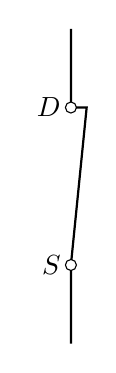
\begin{tikzpicture}
	\draw[thick] (0,0) -- (0,1) node [left] {$S$} -- (0.2,3) -- (0,3) node [left] {$D$} -- (0,4);

	\draw[fill=white] (0,1) circle (0.07);
	\draw[fill=white] (0,3) circle (0.07);
\end{tikzpicture}
\end{lstlisting}

\subsection{11.12.2008-IMG-phys-6}
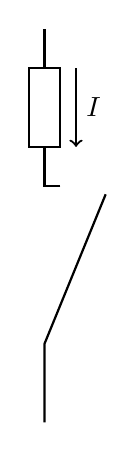
\begin{tikzpicture}
	\draw[thick] (0,0) -- (0,1) -- (75:3);
	\draw[thick] (0.2,3) -- (0,3) -- (0,5);

	\draw[thick, fill=white] (-0.2,3.5) rectangle (0.2,4.5);

	\draw[->, thick] (0.4,4.5) -- (0.4,3.5) node [midway, right] {$I$};
\end{tikzpicture}
\begin{lstlisting}[frame=single]
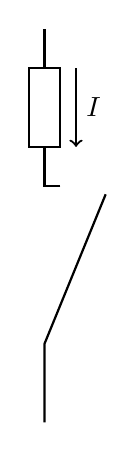
\begin{tikzpicture}
	\draw[thick] (0,0) -- (0,1) -- (75:3);
	\draw[thick] (0.2,3) -- (0,3) -- (0,5);

	\draw[thick, fill=white] (-0.2,3.5) rectangle (0.2,4.5);

	\draw[->, thick] (0.4,4.5) -- (0.4,3.5) node [midway, right] {$I$};
\end{tikzpicture}
\end{lstlisting}

\subsection{11.12.2008-IMG-phys-7}
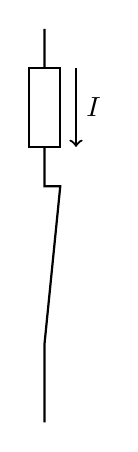
\begin{tikzpicture}
	\draw[thick] (0,0) -- (0,1) -- (0.2,3) -- (0,3) -- (0,5);

	\draw[thick, fill=white] (-0.2,3.5) rectangle (0.2,4.5);

	\draw[->, thick] (0.4,4.5) -- (0.4,3.5) node [midway, right] {$I$};
\end{tikzpicture}
\begin{lstlisting}[frame=single]
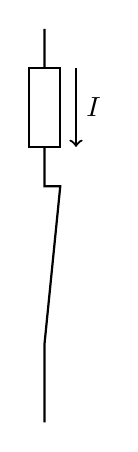
\begin{tikzpicture}
	\draw[thick] (0,0) -- (0,1) -- (0.2,3) -- (0,3) -- (0,5);

	\draw[thick, fill=white] (-0.2,3.5) rectangle (0.2,4.5);

	\draw[->, thick] (0.4,4.5) -- (0.4,3.5) node [midway, right] {$I$};
\end{tikzpicture}
\end{lstlisting}

\section{22.12.2008}
\subsection{22.12.2008-IMG-phys-1}
\begin{tikzpicture}
	\draw[thick, ->] (0,-0.5) -- (0,6) node[left] {$z$};
	\draw[thick, ->] (-0.5,0) -- (8,0) node[below] {$x$};
	\draw[thick, ->] (-0.25,-0.25) -- (4,4) node[right] {$y$};

	\draw[draw=green, ->] (0,0) -- (4.5,-0.5);
	\draw[draw=blue, ->] (0,0) -- (2.5,1.5);
	\draw[draw=red, ->] (0,0) -- (0.5,3);

	\fill[green] (0,0) circle (3pt);
\end{tikzpicture}
\begin{lstlisting}[frame=single]
\begin{tikzpicture}
	\draw[thick, ->] (0,-0.5) -- (0,6) node[left] {$z$};
	\draw[thick, ->] (-0.5,0) -- (8,0) node[below] {$x$};
	\draw[thick, ->] (-0.25,-0.25) -- (4,4) node[right] {$y$};

	\draw[draw=green, ->] (0,0) -- (4.5,-0.5);
	\draw[draw=blue, ->] (0,0) -- (2.5,1.5);
	\draw[draw=red, ->] (0,0) -- (0.5,3);

	\fill[green] (0,0) circle (3pt);
\end{tikzpicture}
\end{lstlisting}

\subsection{22.12.2008-IMG-phys-2}
\begin{tikzpicture}
	\draw[thick, draw=blue, ->] (0,0) -- (0,-7);
	\draw[thick, draw=blue, ->] (2,0) -- (2,-7);
	\draw[thick, draw=blue, ->] (4,0) -- (4,-7);
\end{tikzpicture}
\begin{lstlisting}[frame=single]
\begin{tikzpicture}
	\draw[thick, draw=blue, ->] (0,0) -- (0,-7);
	\draw[thick, draw=blue, ->] (2,0) -- (2,-7);
	\draw[thick, draw=blue, ->] (4,0) -- (4,-7);
\end{tikzpicture}
\end{lstlisting}

\subsection{22.12.2008-IMG-phys-5}
\begin{tikzpicture}
	\draw[thick, dashed, draw=blue] (0,0) rectangle (9,7);
	\draw[thick, draw=blue] (1,1) node[text=blue] {$\times$} circle (0.25);
	\draw[thick, draw=blue] (8,1) node[text=blue] {$\times$} circle (0.25);
	\draw[thick, draw=blue] (1,6) node[text=blue] {$\times$} circle (0.25);
	\draw[thick, draw=blue] (8,6) node[text=blue] {$\times$} circle (0.25);
	\node[text=blue, above] at (4.5,7) {\LARGE{$\vec{B}$}};

	\draw[thick, draw=green!50!black, ->] (-3,5) -- (0,5) node[below, midway, text=green!50!black] {$e^-$-Strahl};
	\draw[thick, draw=green!50!black, dashed] (0,5) -- (4,5);

	\draw[thick] (4,3) circle (2);
	\fill (4,3) circle (1pt);
	\draw[thick, ->] (4,3) -- +(45:2) node[midway, below] {$r$};

	\draw[thick, draw=red, ->] (4,5) -- +(0,-1) node[text=red, left, midway] {$\vec{F_L}$};
	\draw[thick, draw=green!50!black, ->] (4,5) -- +(1,0) node[text=green!50!black, above, midway] {$\vec{v}$};
	\draw[thick, draw=green!50!black, fill=white] (4,5) node[text=green!50!black] {-} circle (3pt);

	\draw[thick, draw=green!50!black, ->] (6,3) -- +(0,-1) node[text=green!50!black, left, midway] {$\vec{v}$};
	\draw[thick, draw=red, ->] (6,3) -- +(-1,0) node[text=red, above, midway] {$\vec{F_L}$};
	\draw[thick, draw=green!50!black, fill=white] (6,3) node[text=green!50!black] {-} circle (3pt);
\end{tikzpicture}
\begin{lstlisting}[frame=single]
\begin{tikzpicture}
	\draw[thick, dashed, draw=blue] (0,0) rectangle (9,7);
	\draw[thick, draw=blue] (1,1) node[text=blue] {$\times$} circle (0.25);
	\draw[thick, draw=blue] (8,1) node[text=blue] {$\times$} circle (0.25);
	\draw[thick, draw=blue] (1,6) node[text=blue] {$\times$} circle (0.25);
	\draw[thick, draw=blue] (8,6) node[text=blue] {$\times$} circle (0.25);
	\node[text=blue, above] at (4.5,7) {\LARGE{$\vec{B}$}};

	\draw[thick, draw=green!50!black, ->] (-3,5) -- (0,5) node[below, midway, text=green!50!black] {$e^-$-Strahl};
	\draw[thick, draw=green!50!black, dashed] (0,5) -- (4,5);

	\draw[thick] (4,3) circle (2);
	\fill (4,3) circle (1pt);
	\draw[thick, ->] (4,3) -- +(45:2) node[midway, below] {$r$};

	\draw[thick, draw=red, ->] (4,5) -- +(0,-1) node[text=red, left, midway] {$\vec{F_L}$};
	\draw[thick, draw=green!50!black, ->] (4,5) -- +(1,0) node[text=green!50!black, above, midway] {$\vec{v}$};
	\draw[thick, draw=green!50!black, fill=white] (4,5) node[text=green!50!black] {-} circle (3pt);

	\draw[thick, draw=green!50!black, ->] (6,3) -- +(0,-1) node[text=green!50!black, left, midway] {$\vec{v}$};
	\draw[thick, draw=red, ->] (6,3) -- +(-1,0) node[text=red, above, midway] {$\vec{F_L}$};
	\draw[thick, draw=green!50!black, fill=white] (6,3) node[text=green!50!black] {-} circle (3pt);
\end{tikzpicture}
\end{lstlisting}

\subsection{22.12.2008-IMG-phys-3}
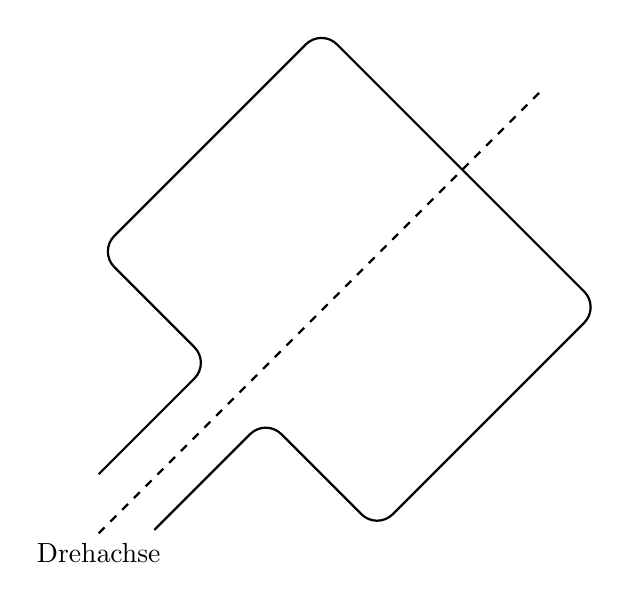
\begin{tikzpicture}
	\draw[thick,rounded corners=8pt] (0,0) -- ++(45:2) -- ++(135:2) -- ++(45:4) -- ++(-45:5) -- ++(-135:4) -- ++(135:2) -- ++(-135:2);
	\draw[thick, dashed] (0,-0.75) node[below] {Drehachse} -- +(45:8);
\end{tikzpicture}
\begin{lstlisting}[frame=single]
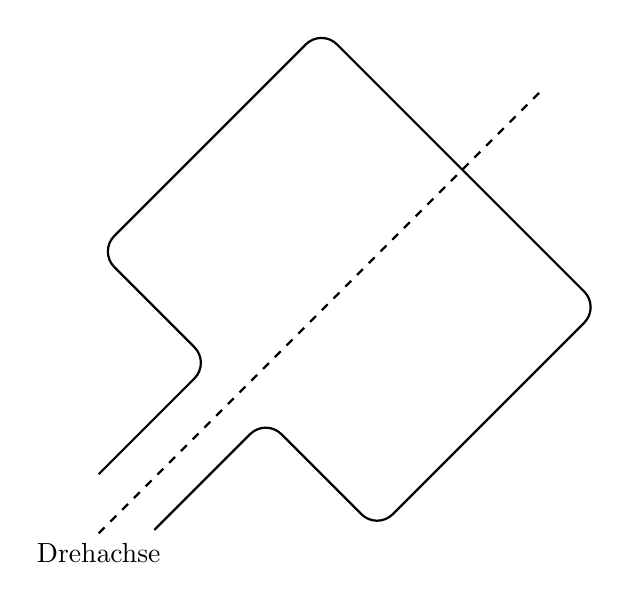
\begin{tikzpicture}
	\draw[thick,rounded corners=8pt] (0,0) -- ++(45:2) -- ++(135:2) -- ++(45:4) -- ++(-45:5) -- ++(-135:4) -- ++(135:2) -- ++(-135:2);
	\draw[thick, dashed] (0,-0.75) node[below] {Drehachse} -- +(45:8);
\end{tikzpicture}
\end{lstlisting}

\section{08.01.2009}
\subsection{08.01.2009-IMG-phys-1}
%Picture
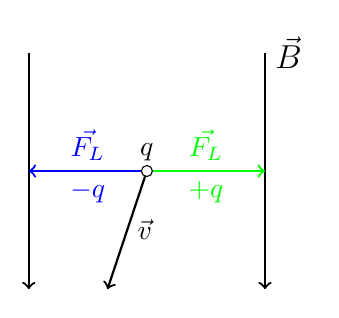
\begin{tikzpicture}
	\draw[->, thick] (0,0) -- (0,-3);
	\draw[->, thick] (3,0) node[right] {\large{$\vec{B}$}} -- (3,-3);

	\draw[->, thick, draw=green] (1.5,-1.5) -- (3,-1.5) node[above, midway, text=green] {$\vec{F_L}$} node[below, midway, text=green] {$+q$};
	\draw[->, thick, draw=blue] (1.5,-1.5) -- (0,-1.5) node[above, midway, text=blue] {$\vec{F_L}$} node[below, midway, text=blue] {$-q$};

	\draw[->, thick] (1.5,-1.5) -- (1,-3) node[right, midway] {$\vec{v}$};

	\draw[fill=white] (1.5,-1.5) circle (0.07) node[above] {$q$};
\end{tikzpicture}
%Code
\begin{lstlisting}[frame=single]
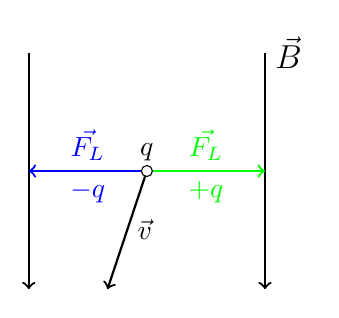
\begin{tikzpicture}
	\draw[->, thick] (0,0) -- (0,-3);
	\draw[->, thick] (3,0) node[right] {\large{$\vec{B}$}} -- (3,-3);

	\draw[->, thick, draw=green] (1.5,-1.5) -- (3,-1.5) node[above, midway, text=green] {$\vec{F_L}$} node[below, midway, text=green] {$+q$};
	\draw[->, thick, draw=blue] (1.5,-1.5) -- (0,-1.5) node[above, midway, text=blue] {$\vec{F_L}$} node[below, midway, text=blue] {$-q$};

	\draw[->, thick] (1.5,-1.5) -- (1,-3) node[right, midway] {$\vec{v}$};

	\draw[fill=white] (1.5,-1.5) circle (0.07) node[above] {$q$};
\end{tikzpicture}
\end{lstlisting}

\section{12.01.2009}
\subsection{12.01.2009-IMG-phys-1}
%Picture
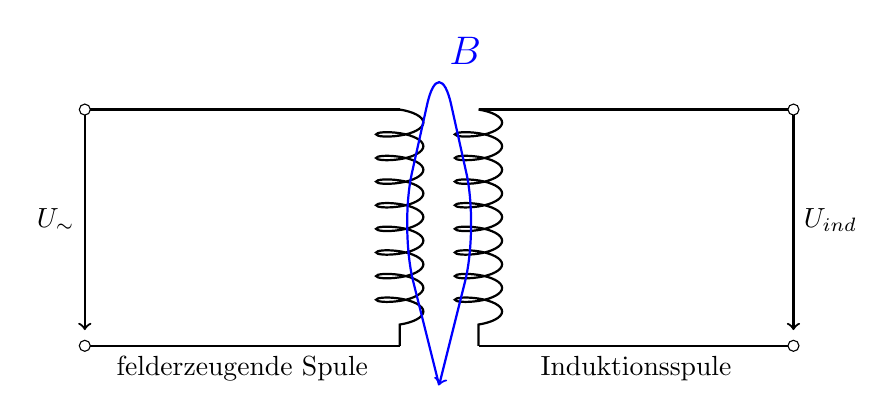
\begin{tikzpicture}[decoration={coil,aspect=0.3,segment length=3mm,amplitude=3mm}]

	%Linker Teil
	\draw[->, thick] (0,0) -- (0,-2.8) node[left, midway] {$U_{\sim}$};
	\draw[thick] (0,0) -- (4,0);
	\draw[thick] (4,-3) -- (0,-3) node[below, midway] {felderzeugende Spule};
	%Spule 1
	\draw[thick, decorate] (4,0) -- (4,-3);

	\draw[fill=white] (0,0) circle (0.07);
	\draw[fill=white] (0,-3) circle (0.07);

	%Rechter Teil
	\draw[thick] (5,0) -- (9,0);
	\draw[->, thick] (9,0) -- (9, -2.8) node[right, midway] {$U_{ind}$};
	\draw[thick] (5,-3) -- (9,-3) node[below, midway] {Induktionsspule};
	%Spule 2
	\draw[thick, decorate] (5,0) -- (5,-3);

	\draw[fill=white] (9,0) circle (0.07);
	\draw[fill=white] (9,-3) circle (0.07);

	\draw[thick, draw=blue, ->, rounded corners=20pt] (4.5,-3.5) -- (4,-1.5) -- (4.5,0.75) node[right, text=blue] {\Large{$B$}} -- (5,-1.5) -- (4.5,-3.5);
\end{tikzpicture}
%Code
\begin{lstlisting}[frame=single]
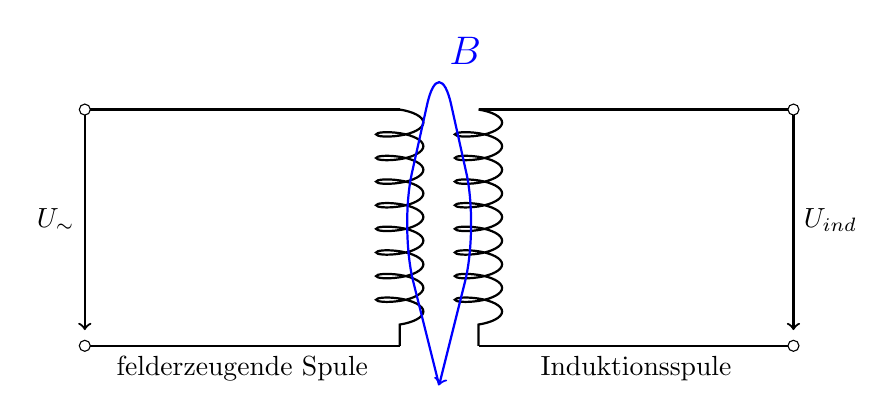
\begin{tikzpicture}[decoration={coil,aspect=0.3,segment length=3mm,amplitude=3mm}]

	%Linker Teil
	\draw[->, thick] (0,0) -- (0,-2.8) node[left, midway] {$U_{\sim}$};
	\draw[thick] (0,0) -- (4,0);
	\draw[thick] (4,-3) -- (0,-3) node[below, midway] {felderzeugende Spule};
	%Spule 1
	\draw[thick, decorate] (4,0) -- (4,-3);

	\draw[fill=white] (0,0) circle (0.07);
	\draw[fill=white] (0,-3) circle (0.07);

	%Rechter Teil
	\draw[thick] (5,0) -- (9,0);
	\draw[->, thick] (9,0) -- (9, -2.8) node[right, midway] {$U_{ind}$};
	\draw[thick] (5,-3) -- (9,-3) node[below, midway] {Induktionsspule};
	%Spule 2
	\draw[thick, decorate] (5,0) -- (5,-3);

	\draw[fill=white] (9,0) circle (0.07);
	\draw[fill=white] (9,-3) circle (0.07);

	\draw[thick, draw=blue, ->, rounded corners=20pt] (4.5,-3.5) -- (4,-1.5) -- (4.5,0.75) node[right, text=blue] {\Large{$B$}} -- (5,-1.5) -- (4.5,-3.5);
\end{tikzpicture}
\end{lstlisting}

\subsection{12.01.2009-IMG-phys-4}
%Picture
\begin{tikzpicture}
	\draw[->, thick] (0,0) node[left] {$B$} -- (0,3) node[left] {$U_N$};
	\draw[->, thick] (-0.2,1.5) node[left] {$I$} -- (5,1.5) node[below] {$t$};
	\draw (0,2.5) -- (5,2.5);
\end{tikzpicture}
%Code
\begin{lstlisting}[frame=single]
\begin{tikzpicture}
	\draw[->, thick] (0,0) node[left] {$B$} -- (0,3) node[left] {$U_N$};
	\draw[->, thick] (-0.2,1.5) node[left] {$I$} -- (5,1.5) node[below] {$t$};
	\draw (0,2.5) -- (5,2.5);
\end{tikzpicture}
\end{lstlisting}

\subsection{12.01.2009-IMG-phys-5}
%Picture
\begin{tikzpicture}
	\draw[->, thick] (0,0) -- (0,3);
	\draw[->, thick] (-0.2,1.5) node[left] {$0$} -- (5,1.5) node[below] {$t$} node[below, midway] {$U_{ind} > 0$};
\end{tikzpicture}
%Code
\begin{lstlisting}[frame=single]
\begin{tikzpicture}
	\draw[->, thick] (0,0) -- (0,3);
	\draw[->, thick] (-0.2,1.5) node[left] {$0$} -- (5,1.5) node[below] {$t$} node[below, midway] {$U_{ind} > 0$};
\end{tikzpicture}
\end{lstlisting}

%\chapter{Mathematik}
\section{05.11.2008}
\subsection{05.11.2008-IMG-mathe-4}
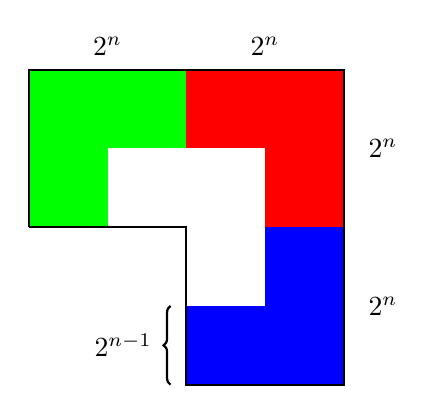
\begin{tikzpicture}[thick]
	\fill[fill=green] (0,0) rectangle (1,2);
	\fill[fill=green] (1,2) rectangle (2,1);

	\fill[fill=red] (2,2) rectangle (4,1);
	\fill[fill=red] (3,1) rectangle (4,0);

	\fill[fill=blue] (3,0) rectangle (4,-2);
	\fill[fill=blue] (3,-2) rectangle (2,-1);

	\draw (0,0) -- (2,0) -- (2,-2) -- (4,-2) -- (4,2) -- (0,2) -- (0,0);

	\node at (1,2.3) {$2^n$};
	\node at (3,2.3) {$2^n$};
	\node at (4.5,1) {$2^n$};
	\node at (4.5,-1) {$2^n$};
	\draw decorate [decoration=brace] {(1.8,-2) -- (1.8,-1)};
	\node at (1.2,-1.5) {$2^{n-1}$};
\end{tikzpicture}
\begin{lstlisting}[frame=single]
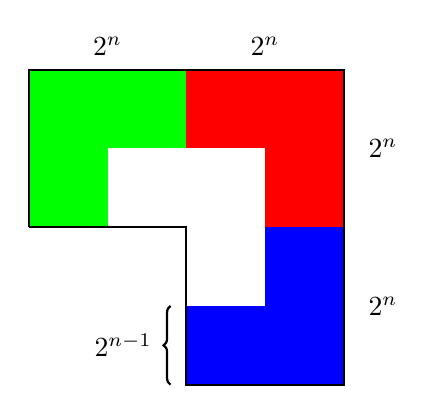
\begin{tikzpicture}[thick]
	\fill[fill=green] (0,0) rectangle (1,2);
	\fill[fill=green] (1,2) rectangle (2,1);

	\fill[fill=red] (2,2) rectangle (4,1);
	\fill[fill=red] (3,1) rectangle (4,0);

	\fill[fill=blue] (3,0) rectangle (4,-2);
	\fill[fill=blue] (3,-2) rectangle (2,-1);

	\draw (0,0) -- (2,0) -- (2,-2) -- (4,-2) -- (4,2) -- (0,2) -- (0,0);

	\node at (1,2.3) {$2^n$};
	\node at (3,2.3) {$2^n$};
	\node at (4.5,1) {$2^n$};
	\node at (4.5,-1) {$2^n$};
	\draw decorate [decoration=brace] {(1.8,-2) -- (1.8,-1)};
	\node at (1.2,-1.5) {$2^{n-1}$};
\end{tikzpicture}
\end{lstlisting}

\subsection{05.11.2008-IMG-mathe-5}
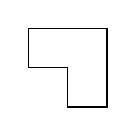
\begin{tikzpicture}
	\draw (0,0) -- (0,0.5) -- (1,0.5) -- (1,-0.5) -- (0.5,-0.5) -- (0.5,0) -- (0,0);
\end{tikzpicture}
\begin{lstlisting}[frame=single]
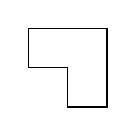
\begin{tikzpicture}
	\draw (0,0) -- (0,0.5) -- (1,0.5) -- (1,-0.5) -- (0.5,-0.5) -- (0.5,0) -- (0,0);
\end{tikzpicture}
\end{lstlisting}

\subsection{05.11.2008-IMG-mathe-6}
\begin{tikzpicture}
	\draw (0,0) rectangle (0.5,0.5);

	\node at (0.25,0.8) {$1$};
	\node at (0.8,0.25) {$1$};
\end{tikzpicture}
\begin{lstlisting}[frame=single]
\begin{tikzpicture}
	\draw (0,0) rectangle (0.5,0.5);

	\node at (0.25,0.8) {$1$};
	\node at (0.8,0.25) {$1$};
\end{tikzpicture}
\end{lstlisting}

\subsection{05.11.2008-IMG-mathe-7}
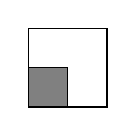
\begin{tikzpicture}
	\draw (0,0) rectangle (1,1);
	\draw[fill=gray] (0,0) rectangle (0.5,0.5);
\end{tikzpicture}
\begin{lstlisting}[frame=single]
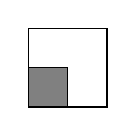
\begin{tikzpicture}
	\draw (0,0) rectangle (1,1);
	\draw[fill=gray] (0,0) rectangle (0.5,0.5);
\end{tikzpicture}
\end{lstlisting}

\subsection{05.11.2008-IMG-mathe-8}
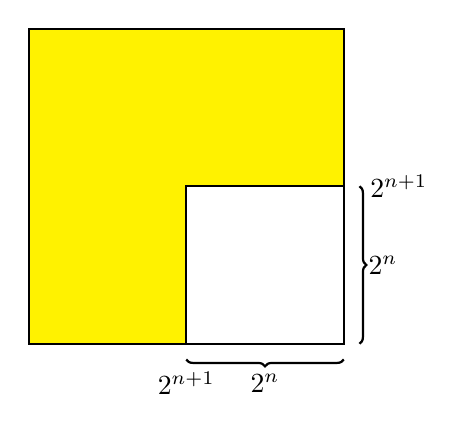
\begin{tikzpicture}[thick]
	\draw[fill=yellow] (0,0) rectangle (4,4);
	\draw[fill=white] (2,2) rectangle (4,0);

	\draw decorate [decoration=brace]  {(4,-0.2) -- (2,-0.2)};
	\draw decorate [decoration=brace] {(4.2,2) -- (4.2,0)};

	\node at (2,-0.5) {$2^{n+1}$};
	\node at (4.7,2) {$2^{n+1}$};
	\node at (3,-0.5) {$2^n$};
	\node at (4.5,1) {$2^n$};
\end{tikzpicture}
\begin{lstlisting}[frame=single]
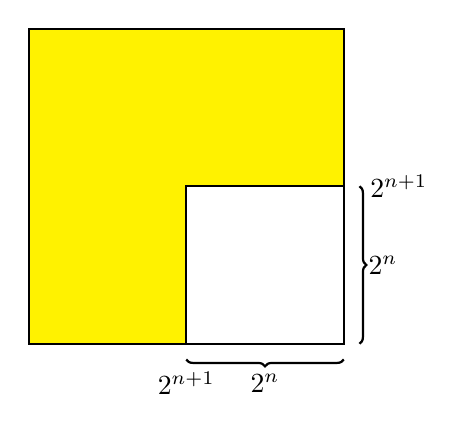
\begin{tikzpicture}[thick]
	\draw[fill=yellow] (0,0) rectangle (4,4);
	\draw[fill=white] (2,2) rectangle (4,0);

	\draw decorate [decoration=brace]  {(4,-0.2) -- (2,-0.2)};
	\draw decorate [decoration=brace] {(4.2,2) -- (4.2,0)};

	\node at (2,-0.5) {$2^{n+1}$};
	\node at (4.7,2) {$2^{n+1}$};
	\node at (3,-0.5) {$2^n$};
	\node at (4.5,1) {$2^n$};
\end{tikzpicture}
\end{lstlisting}

\subsection{05.11.2008-IMG-mathe-9}

\begin{tikzpicture}
	\fill[fill=yellow] (0,0) rectangle (0.5,1);
	\fill[fill=yellow] (0.5,1) rectangle (1,0.5);
	\draw (0,0) -- (0,1) -- (1,1) -- (1,0.5) -- (0.5,0.5) -- (0.5,0) -- (0,0);
\end{tikzpicture}
\begin{lstlisting}[frame=single]

\begin{tikzpicture}
	\fill[fill=yellow] (0,0) rectangle (0.5,1);
	\fill[fill=yellow] (0.5,1) rectangle (1,0.5);
	\draw (0,0) -- (0,1) -- (1,1) -- (1,0.5) -- (0.5,0.5) -- (0.5,0) -- (0,0);
\end{tikzpicture}
\end{lstlisting}

\subsection{05.11.2008-IMG-mathe-10}
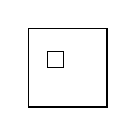
\begin{tikzpicture}
	\draw (0,0) rectangle (1,1);
	\draw (0.25,0.5) rectangle (0.45,0.7);
\end{tikzpicture}
\begin{lstlisting}[frame=single]
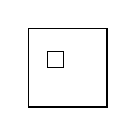
\begin{tikzpicture}
	\draw (0,0) rectangle (1,1);
	\draw (0.25,0.5) rectangle (0.45,0.7);
\end{tikzpicture}
\end{lstlisting}

\subsection{IMG-05.11.2008-mathe-3}
\begin{tikzpicture}
	\draw (0,0) -- (2,0) -- (2,-2) -- (4,-2) -- (4,2) -- (0,2) -- (0,0);

	\draw[dashed] (2,0) -- (2,2);
	\draw[dashed] (2,0) -- (4,0);

	\node at (1,2.3) {$2^{n-1}$};
	\node at (3,2.3) {$2^{n-1}$};
	\node at (4.5,1) {$2^{n-1}$};
	\node at (4.5,-1) {$2^{n-1}$};
\end{tikzpicture}
\begin{lstlisting}[frame=single]
\begin{tikzpicture}
	\draw (0,0) -- (2,0) -- (2,-2) -- (4,-2) -- (4,2) -- (0,2) -- (0,0);

	\draw[dashed] (2,0) -- (2,2);
	\draw[dashed] (2,0) -- (4,0);

	\node at (1,2.3) {$2^{n-1}$};
	\node at (3,2.3) {$2^{n-1}$};
	\node at (4.5,1) {$2^{n-1}$};
	\node at (4.5,-1) {$2^{n-1}$};
\end{tikzpicture}
\end{lstlisting}

\section{11.12.2008}
\subsection{11.12.2008-IMG-mathe-1}
\definecolor{lightergray}{HTML}{DDDDDD}
\begin{tikzpicture}
	\draw[fill=lightergray, line width=0pt, draw=lightergray] (0,0) -- (1.5,2) -- (4.5,2.5) -- (3,0.5) -- (0,0);

	\draw[->] (0,0) -- (1.5,2) node[left] {$\vec{v_2}$};
	\draw[->] (0,0) -- (3,0.5) node[below] {$\vec{v_1}$};

	\draw[->, thick] (-0.5,0) -- (5.5,0) node[below] {$x$};
	\draw[->, thick] (0,-0.5) -- (0,3) node[left] {$y$};
\end{tikzpicture}
\begin{lstlisting}[frame=single]
\definecolor{lightergray}{HTML}{DDDDDD}
\begin{tikzpicture}
	\draw[fill=lightergray, line width=0pt, draw=lightergray] (0,0) -- (1.5,2) -- (4.5,2.5) -- (3,0.5) -- (0,0);

	\draw[->] (0,0) -- (1.5,2) node[left] {$\vec{v_2}$};
	\draw[->] (0,0) -- (3,0.5) node[below] {$\vec{v_1}$};

	\draw[->, thick] (-0.5,0) -- (5.5,0) node[below] {$x$};
	\draw[->, thick] (0,-0.5) -- (0,3) node[left] {$y$};
\end{tikzpicture}
\end{lstlisting}

\subsection{11.12.2008-IMG-mathe-2}
\begin{tikzpicture}
	\draw[fill=lightergray] (2,3) -- (3.5,0) -- (5,3) -- (2,3); 

	\draw[fill=yellow, line width=0pt, draw=yellow] (0,0) -- (2,3) -- (3.5,0) -- (0,0);

	\draw[->] (0,0) -- (2,3) node[left] {$\vec{v_2}$};
	\draw[->, thick] (0,0) -- (3.5,0) node[below] {$\vec{v_1}$};
	\draw (1.25,0) -- (1,-0.25) node[below] {$s$};
	\draw[<->] (5,3) -- (5,0);
	\node[right] at (5,1.5) {$h$};

	\draw[->, thick] (-0.5,0) -- (5.5,0) node[below] {$x$};
	\draw[->, thick] (0,-0.5) -- (0,3) node[left] {$y$};
\end{tikzpicture}
\begin{lstlisting}[frame=single]
\begin{tikzpicture}
	\draw[fill=lightergray] (2,3) -- (3.5,0) -- (5,3) -- (2,3); 

	\draw[fill=yellow, line width=0pt, draw=yellow] (0,0) -- (2,3) -- (3.5,0) -- (0,0);

	\draw[->] (0,0) -- (2,3) node[left] {$\vec{v_2}$};
	\draw[->, thick] (0,0) -- (3.5,0) node[below] {$\vec{v_1}$};
	\draw (1.25,0) -- (1,-0.25) node[below] {$s$};
	\draw[<->] (5,3) -- (5,0);
	\node[right] at (5,1.5) {$h$};

	\draw[->, thick] (-0.5,0) -- (5.5,0) node[below] {$x$};
	\draw[->, thick] (0,-0.5) -- (0,3) node[left] {$y$};
\end{tikzpicture}
\end{lstlisting}

\subsection{11.12.2008-IMG-mathe-3}
\begin{tikzpicture}
	\draw[->, thick] (0,0) -- (6,0) node[right] {$y$};
	\draw[->, thick] (0,0) -- (0,7) node[left] {$z$};
	\draw[->, thick] (0,0) -- (-2,-2.5) node[below] {$x$};

	\draw[draw=gray, nearly opaque, thick] (-1,-2) -- (-1,4) -- (2,4) -- (2,-2) -- (-1,-2);
	\draw[draw=gray, nearly opaque, thick] (-1,4) -- (1,6) -- (4,6) -- (2,4);
	\draw[draw=gray, nearly opaque, thick] (2,-2) -- (4,0) -- (4,6) node [above] {\LARGE{$V$}};
\end{tikzpicture}
\begin{lstlisting}[frame=single]
\begin{tikzpicture}
	\draw[->, thick] (0,0) -- (6,0) node[right] {$y$};
	\draw[->, thick] (0,0) -- (0,7) node[left] {$z$};
	\draw[->, thick] (0,0) -- (-2,-2.5) node[below] {$x$};

	\draw[draw=gray, nearly opaque, thick] (-1,-2) -- (-1,4) -- (2,4) -- (2,-2) -- (-1,-2);
	\draw[draw=gray, nearly opaque, thick] (-1,4) -- (1,6) -- (4,6) -- (2,4);
	\draw[draw=gray, nearly opaque, thick] (2,-2) -- (4,0) -- (4,6) node [above] {\LARGE{$V$}};
\end{tikzpicture}
\end{lstlisting}

\section{08.01.2009}
\subsection{08.01.2009-IMG-math-1}
%Picture
\begin{tikzpicture}
	\node at (0,0) (Vl) {$V$};
	\node at (3,0) (Vr) {$V$};
	\node at (0,3) (Kl) {$K^n$};
	\node at (3,3) (Kr) {$K^n$};

	\draw[->] (Vl.north) -- (Kl.south);
	\draw[->] (Vl.east) -- (Vr.west) node[above, midway] {$f$};

	\draw[->] (Kl.east) -- (Kr.west) node[below, midway] {$f$};

	\draw[->] (Kr.south) -- (Vr.north);
\end{tikzpicture}
%Code
\begin{lstlisting}[frame=single]
\begin{tikzpicture}
	\node at (0,0) (Vl) {$V$};
	\node at (3,0) (Vr) {$V$};
	\node at (0,3) (Kl) {$K^n$};
	\node at (3,3) (Kr) {$K^n$};

	\draw[->] (Vl.north) -- (Kl.south);
	\draw[->] (Vl.east) -- (Vr.west) node[above, midway] {$f$};

	\draw[->] (Kl.east) -- (Kr.west) node[below, midway] {$f$};

	\draw[->] (Kr.south) -- (Vr.north);
\end{tikzpicture}
\end{lstlisting}

\section{14.01.2009}
\subsection{14.01.2009-IMG-mathe-1}
%Picture
\begin{tikzpicture}
	\draw[thick, <->] (3,0) -- (0,0) -- (0,3);

	\draw[->] (0,0) -- (2,2) node[left, midway] {$\vec{v}$};
	\draw[draw=blue, thick] (0,0) -- (2,0) node[below, midway, text=blue] {$U_1$};
	\draw[draw=blue] (2,0) -- (2,2) node[right, midway, text=blue] {$U_2$};
	\draw[draw=blue] (1.7,0) arc (180:90:0.3);
	\draw[draw=blue, fill=blue] (1.9,0.125) circle (0.02);
\end{tikzpicture}
%Code
\begin{lstlisting}[frame=single]
\begin{tikzpicture}
	\draw[thick, <->] (3,0) -- (0,0) -- (0,3);

	\draw[->] (0,0) -- (2,2) node[left, midway] {$\vec{v}$};
	\draw[draw=blue, thick] (0,0) -- (2,0) node[below, midway, text=blue] {$U_1$};
	\draw[draw=blue] (2,0) -- (2,2) node[right, midway, text=blue] {$U_2$};
	\draw[draw=blue] (1.7,0) arc (180:90:0.3);
	\draw[draw=blue, fill=blue] (1.9,0.125) circle (0.02);
\end{tikzpicture}
\end{lstlisting}

\subsection{14.01.2009-IMG-mathe-2}
%Picture
\begin{tikzpicture}
	\draw[->, thick] (0,0) -- (3,0) node[below, midway] {$\vec{u}$};
	\draw[->, thick] (0,0) -- (45:1.5) node[left, midway] {$\vec{r}$};
	\draw[thick] (0.8,0) arc (0:45:0.8);
	\path (0,0) ++(22.5:0.5) node{$\alpha$};
\end{tikzpicture}
%Code
\begin{lstlisting}[frame=single]
\begin{tikzpicture}
	\draw[->, thick] (0,0) -- (3,0) node[below, midway] {$\vec{u}$};
	\draw[->, thick] (0,0) -- (45:1.5) node[left, midway] {$\vec{r}$};
	\draw[thick] (0.8,0) arc (0:45:0.8);
	\path (0,0) ++(22.5:0.5) node{$\alpha$};
\end{tikzpicture}
\end{lstlisting}

\subsection{14.01.2009-IMG-mathe-3}
%Picture
\begin{tikzpicture}
	\draw[->, thick] (0,0) -- (3,0) node[below, midway] {$\vec{u}$};
	\draw[->, thick] (0,0) -- (45:1.5) node[left, midway] {$\vec{v}$};
	\draw[thick] (0.8,0) arc (0:45:0.8);
	\path (0,0) ++(22.5:0.5) node{$\alpha$};
\end{tikzpicture}
%Code
\begin{lstlisting}[frame=single]
\begin{tikzpicture}
	\draw[->, thick] (0,0) -- (3,0) node[below, midway] {$\vec{u}$};
	\draw[->, thick] (0,0) -- (45:1.5) node[left, midway] {$\vec{v}$};
	\draw[thick] (0.8,0) arc (0:45:0.8);
	\path (0,0) ++(22.5:0.5) node{$\alpha$};
\end{tikzpicture}
\end{lstlisting}

\subsection{14.01.2009-IMG-mathe-4}
%Picture
\begin{tikzpicture}
	\draw[->, thick] (-1.5,0) -- (1.5,0) node[below] {$x$};
	\draw[->, thick] (0,-0.5) -- (0,1);
	\draw[smooth] plot[domain=-3:3, scale=0.5] (\x,{cos(\x r)});
\end{tikzpicture}
%Code
\begin{lstlisting}[frame=single]
\begin{tikzpicture}
	\draw[->, thick] (-1.5,0) -- (1.5,0) node[below] {$x$};
	\draw[->, thick] (0,-0.5) -- (0,1);
	\draw[smooth] plot[domain=-3:3, scale=0.5] (\x,{cos(\x r)});
\end{tikzpicture}
\end{lstlisting}

\section{15.01.2009}
\subsection{15.01.2009-IMG-mathe-1}
%Picture
\begin{tikzpicture}
	\draw[<->, thick] (0,3) -- (0,0) node[left, midway] {$\vec{v}$} -- (5,0) node[below, midway] {$\vec{u}$};
	\draw[thick] (0,0.5) arc (90:0:0.5);
	\path (0,0) ++(45:0.25) node{$\alpha$};
\end{tikzpicture}
%Code
\begin{lstlisting}[frame=single]
\begin{tikzpicture}
	\draw[<->, thick] (0,3) -- (0,0) node[left, midway] {$\vec{v}$} -- (5,0) node[below, midway] {$\vec{u}$};
	\draw[thick] (0,0.5) arc (90:0:0.5);
	\path (0,0) ++(45:0.25) node{$\alpha$};
\end{tikzpicture}
\end{lstlisting}

\subsection{15.01.2009-IMG-mathe-2}
%Picture
\begin{tikzpicture}
	\draw[->, thick] (0,0) -- (3,3) node[left, midway] {$\vec{u} + \vec{v}$};
	\draw[->, thick] (0,0) -- (3,0) node[below, midway] {$\vec{u}$};
	\draw[->, thick] (3,0) -- (3,3) node[right, midway] {$\vec{v}$};
\end{tikzpicture}
%Code
\begin{lstlisting}[frame=single]
\begin{tikzpicture}
	\draw[->, thick] (0,0) -- (3,3) node[left, midway] {$\vec{u} + \vec{v}$};
	\draw[->, thick] (0,0) -- (3,0) node[below, midway] {$\vec{u}$};
	\draw[->, thick] (3,0) -- (3,3) node[right, midway] {$\vec{v}$};
\end{tikzpicture}
\end{lstlisting}

\subsection{15.01.2009-IMG-mathe-3}
%Picture
\begin{tikzpicture}
	\draw[thick] (0,0) -- (45:4);
	\draw[thick] (45:2) -- +(135:1);
	\draw[fill=black] (45:2) ++ (135:1) circle (0.04) node[left] {$A$};
	\draw[thick] (45:2) ++ (135:0.5) arc (135:45:0.5);
	\draw[fill=black] (45:2) ++ (90:0.25) circle (0.04);
\end{tikzpicture}
%Code
\begin{lstlisting}[frame=single]
\begin{tikzpicture}
	\draw[thick] (0,0) -- (45:4);
	\draw[thick] (45:2) -- +(135:1);
	\draw[fill=black] (45:2) ++ (135:1) circle (0.04) node[left] {$A$};
	\draw[thick] (45:2) ++ (135:0.5) arc (135:45:0.5);
	\draw[fill=black] (45:2) ++ (90:0.25) circle (0.04);
\end{tikzpicture}
\end{lstlisting}


\part{Allgemein}
\chapter{Logos}
\section{FH-Regensburg}
%Picture
%LaTeX with PSTricks extensions
%%Creator: 0.46
%%Please note this file requires PSTricks extensions
\psset{xunit=.5pt,yunit=.5pt,runit=.5pt}
\begin{pspicture}(744.09448242,1052.36218262)
{
\newrgbcolor{curcolor}{1 1 1}
\pscustom[linestyle=none,fillstyle=solid,fillcolor=curcolor]
{
\newpath
\moveto(394.24151735,936.52025422)
\lineto(506.3845151,936.52025422)
\lineto(506.3845151,824.37725648)
\lineto(394.24151735,824.37725648)
\lineto(394.24151735,936.52025422)
\closepath
}
}
{
\newrgbcolor{curcolor}{0 0 0}
\pscustom[linewidth=1,linecolor=curcolor]
{
\newpath
\moveto(394.24151735,936.52025422)
\lineto(506.3845151,936.52025422)
\lineto(506.3845151,824.37725648)
\lineto(394.24151735,824.37725648)
\lineto(394.24151735,936.52025422)
\closepath
}
}
{
\newrgbcolor{curcolor}{0 0 0}
\pscustom[linestyle=none,fillstyle=solid,fillcolor=curcolor]
{
\newpath
\moveto(394.23834353,824.52342805)
\lineto(506.38767366,824.52342805)
\lineto(506.38767366,713.80267152)
\lineto(394.23834353,713.80267152)
\lineto(394.23834353,824.52342805)
\closepath
}
}
{
\newrgbcolor{curcolor}{0 0 0}
\pscustom[linewidth=0.99366665,linecolor=curcolor]
{
\newpath
\moveto(394.23834353,824.52342805)
\lineto(506.38767366,824.52342805)
\lineto(506.38767366,713.80267152)
\lineto(394.23834353,713.80267152)
\lineto(394.23834353,824.52342805)
\closepath
}
}
{
\newrgbcolor{curcolor}{0 0 0}
\pscustom[linestyle=none,fillstyle=solid,fillcolor=curcolor]
{
\newpath
\moveto(393.91536144,867.47575804)
\curveto(403.1466392,867.47575804)(410.63869071,859.98370653)(410.63869071,850.75242877)
\curveto(410.63869071,841.52115101)(403.1466392,834.0290995)(393.91536144,834.0290995)
\curveto(393.91536117,834.0290995)(393.91536094,834.0290995)(393.91536066,834.0290995)
\lineto(393.91536144,850.75242877)
\lineto(393.91536144,867.47575804)
\closepath
}
}
{
\newrgbcolor{curcolor}{0 0 0}
\pscustom[linewidth=0.7676282,linecolor=curcolor]
{
\newpath
\moveto(393.91536144,867.47575804)
\curveto(403.1466392,867.47575804)(410.63869071,859.98370653)(410.63869071,850.75242877)
\curveto(410.63869071,841.52115101)(403.1466392,834.0290995)(393.91536144,834.0290995)
\curveto(393.91536117,834.0290995)(393.91536094,834.0290995)(393.91536066,834.0290995)
\lineto(393.91536144,850.75242877)
\lineto(393.91536144,867.47575804)
\closepath
}
}
{
\newrgbcolor{curcolor}{1 1 1}
\pscustom[linestyle=none,fillstyle=solid,fillcolor=curcolor]
{
\newpath
\moveto(400.4913,809.11405262)
\lineto(408.70558,813.22119262)
\curveto(444.34302,740.49108262)(418.41253,758.52926262)(449.33058,721.07832262)
\lineto(443.34844,715.36404262)
\curveto(412.7532,744.17357262)(431.08654,751.37595262)(400.4913,809.11405262)
\closepath
}
}
{
\newrgbcolor{curcolor}{0 0 0}
\pscustom[linewidth=1,linecolor=curcolor]
{
\newpath
\moveto(400.4913,809.11405262)
\lineto(408.70558,813.22119262)
\curveto(444.34302,740.49108262)(418.41253,758.52926262)(449.33058,721.07832262)
\lineto(443.34844,715.36404262)
\curveto(412.7532,744.17357262)(431.08654,751.37595262)(400.4913,809.11405262)
\closepath
}
}
{
\newrgbcolor{curcolor}{0 0 0}
\pscustom[linestyle=none,fillstyle=solid,fillcolor=curcolor]
{
\newpath
\moveto(378.57977505,811.47862824)
\lineto(378.57977505,824.03599385)
\lineto(369.52505742,838.75456778)
\lineto(372.50603442,838.75456778)
\lineto(379.82805917,826.25309549)
\lineto(387.18734614,838.75456778)
\lineto(390.01927429,838.75456778)
\lineto(381.05771218,824.03599385)
\lineto(381.05771218,811.47862824)
\lineto(378.57977505,811.47862824)
\closepath
}
}
{
\newrgbcolor{curcolor}{0 0 0}
\pscustom[linestyle=none,fillstyle=solid,fillcolor=curcolor]
{
\newpath
\moveto(168.06891739,910.03816804)
\lineto(168.06891739,937.31410758)
\lineto(170.54685452,937.31410758)
\lineto(170.54685452,926.24723047)
\lineto(185.39584619,926.24723047)
\lineto(185.39584619,937.31410758)
\lineto(187.87378332,937.31410758)
\lineto(187.87378332,910.03816804)
\lineto(185.39584619,910.03816804)
\lineto(185.39584619,924.12328436)
\lineto(170.54685452,924.12328436)
\lineto(170.54685452,910.03816804)
\lineto(168.06891739,910.03816804)
\closepath
}
}
{
\newrgbcolor{curcolor}{0 0 0}
\pscustom[linestyle=none,fillstyle=solid,fillcolor=curcolor]
{
\newpath
\moveto(243.83777142,932.37681827)
\curveto(242.48388709,933.54434415)(241.09897624,934.40758454)(239.68303473,934.96654204)
\curveto(238.26705093,935.52544979)(236.77656392,935.80491611)(235.21156923,935.80494182)
\curveto(231.68406664,935.80491611)(228.81798433,934.68705085)(226.6133137,932.4513427)
\curveto(224.40862692,930.21558983)(223.30628757,927.3029298)(223.30629234,923.71335387)
\curveto(223.30628757,921.91233511)(223.57643834,920.29143049)(224.11674547,918.85063514)
\curveto(224.65704143,917.40982227)(225.47991446,916.13048759)(226.58536704,915.01262725)
\curveto(227.6783828,913.91959853)(228.92977085,913.08740995)(230.33953495,912.51605902)
\curveto(231.74927544,911.94470324)(233.26149872,911.65902656)(234.87620932,911.65902813)
\curveto(236.44120434,911.65902656)(237.96895352,911.92607215)(239.45946146,912.4601657)
\curveto(240.94992754,912.99425451)(242.35967984,913.78297055)(243.68872257,914.82631619)
\lineto(243.68872257,911.91986362)
\curveto(242.34725911,911.10009394)(240.92819127,910.46974214)(239.4315148,910.02880633)
\curveto(237.93479653,909.58787066)(236.45362507,909.36740279)(234.98799596,909.36740206)
\curveto(233.01308422,909.36740279)(231.12513401,909.72139345)(229.32413966,910.42937512)
\curveto(227.52312374,911.13735611)(225.97674347,912.13101412)(224.68499421,913.41035212)
\curveto(223.35597047,914.72694566)(222.34989174,916.25469484)(221.66675499,917.99360425)
\curveto(220.98361199,919.73249786)(220.64204205,921.63907916)(220.64204415,923.71335387)
\curveto(220.64204205,925.75033916)(220.99292753,927.6507101)(221.69470165,929.41447238)
\curveto(222.39646946,931.17819602)(223.40565337,932.69973484)(224.72225642,933.97909341)
\curveto(226.00158492,935.23356276)(227.54486001,936.21480004)(229.35208632,936.92280819)
\curveto(231.159291,937.63076269)(233.03792567,937.98475336)(234.98799596,937.98478125)
\curveto(236.72688102,937.98475336)(238.3384701,937.7456544)(239.82276803,937.26748366)
\curveto(241.30702339,936.78925857)(242.65777724,936.0719617)(243.87503364,935.11559089)
\lineto(243.83777142,932.37681827)
\closepath
}
}
{
\newrgbcolor{curcolor}{0 0 0}
\pscustom[linestyle=none,fillstyle=solid,fillcolor=curcolor]
{
\newpath
\moveto(204.90698854,911.5845037)
\curveto(206.52166613,911.58450221)(208.04941531,911.88259962)(209.49024068,912.4787968)
\curveto(210.93102353,913.07498922)(212.2289893,913.94443998)(213.38414188,915.08715168)
\curveto(214.51440271,916.24227412)(215.38074829,917.55576579)(215.98318121,919.02763065)
\curveto(216.58555862,920.49947764)(216.8867612,922.04896309)(216.88678986,923.67609166)
\curveto(216.8867612,925.31561378)(216.5886638,926.86509924)(215.99249676,928.32455266)
\curveto(215.39627419,929.78396963)(214.52682344,931.09746131)(213.38414188,932.26503163)
\curveto(212.25383075,933.40771617)(210.96518052,934.27716692)(209.51818734,934.87338651)
\curveto(208.07115158,935.46955653)(206.53408685,935.76765393)(204.90698854,935.76767961)
\curveto(203.29227761,935.76765393)(201.77073879,935.46955653)(200.34236751,934.87338651)
\curveto(198.91397202,934.27716692)(197.62221661,933.40771617)(196.46709742,932.26503163)
\curveto(195.32438247,931.08504058)(194.45493172,929.7715489)(193.85874254,928.32455266)
\curveto(193.26254211,926.87751996)(192.96444471,925.32803451)(192.96444944,923.67609166)
\curveto(192.96444471,922.03654236)(193.26254211,920.48705691)(193.85874254,919.02763065)
\curveto(194.45493172,917.56818652)(195.32438247,916.25469484)(196.46709742,915.08715168)
\curveto(197.60979589,913.93201925)(198.88913057,913.05946332)(200.3051053,912.46948125)
\curveto(201.72105589,911.87949443)(203.25501543,911.58450221)(204.90698854,911.5845037)
\lineto(204.90698854,911.5845037)
\closepath
\moveto(219.51377584,923.67609166)
\curveto(219.51374456,921.75086569)(219.14733317,919.92191392)(218.41454057,918.18923087)
\curveto(217.68168761,916.45653162)(216.62592598,914.91325653)(215.24725251,913.55940097)
\curveto(213.84368356,912.19311774)(212.26004111,911.15288202)(210.49632042,910.43869067)
\curveto(208.73255519,909.72449863)(206.86944643,909.36740279)(204.90698854,909.36740206)
\curveto(202.94449731,909.36740279)(201.08449373,909.72449863)(199.32697222,910.43869067)
\curveto(197.56942853,911.15288202)(195.99510163,912.19311774)(194.60398679,913.55940097)
\curveto(193.21285921,914.93809798)(192.1539924,916.48758344)(191.42738318,918.20786197)
\curveto(190.70076757,919.92812428)(190.33746136,921.75086569)(190.33746346,923.67609166)
\curveto(190.33746136,925.62613191)(190.70076757,927.4675044)(191.42738318,929.20021466)
\curveto(192.1539924,930.9328867)(193.21285921,932.48858251)(194.60398679,933.86730677)
\curveto(195.97026018,935.22114203)(197.52906118,936.24585185)(199.28039446,936.9414393)
\curveto(201.03170565,937.63697306)(202.90723513,937.98475336)(204.90698854,937.98478125)
\curveto(206.91912933,937.98475336)(208.80397436,937.63386788)(210.56152929,936.93212375)
\curveto(212.31903956,936.23032594)(213.88094574,935.20872131)(215.24725251,933.86730677)
\curveto(216.6383467,932.48858251)(217.69721351,930.9328867)(218.42385612,929.20021466)
\curveto(219.15043835,927.4675044)(219.51374456,925.62613191)(219.51377584,923.67609166)
\lineto(219.51377584,923.67609166)
\closepath
}
}
{
\newrgbcolor{curcolor}{0 0 0}
\pscustom[linestyle=none,fillstyle=solid,fillcolor=curcolor]
{
\newpath
\moveto(371.06894493,764.64517133)
\lineto(374.25771084,764.64517133)
\curveto(376.83826961,764.64516919)(378.66853983,764.80353343)(379.74852699,765.12026452)
\curveto(380.82848605,765.43699037)(381.74362116,765.9741867)(382.49393507,766.73185512)
\curveto(383.53978697,767.80003319)(384.32987256,769.1290507)(384.86419421,770.71891164)
\curveto(385.39847753,772.30875614)(385.66562878,774.12218191)(385.66564875,776.15919436)
\curveto(385.66562878,778.24586241)(385.3956355,780.08412962)(384.8556681,781.67400151)
\curveto(384.31566239,783.26383506)(383.51705069,784.56801113)(382.45983062,785.58653361)
\curveto(381.66404419,786.36901616)(380.69206839,786.9217384)(379.5439003,787.24470198)
\curveto(378.39570451,787.56761607)(376.38922815,787.72908549)(373.5244652,787.72911071)
\lineto(373.0981596,787.72911071)
\lineto(371.06894493,787.72911071)
\lineto(371.06894493,764.64517133)
\closepath
\moveto(368.80099913,762.50259423)
\lineto(368.80099913,789.77853229)
\lineto(372.68890622,789.77853229)
\curveto(376.15618132,789.77850501)(378.61738321,789.59219415)(380.07251925,789.21959913)
\curveto(381.52762654,788.84695068)(382.77812172,788.20728338)(383.82400854,787.30059529)
\curveto(385.21090326,786.09576023)(386.26814009,784.54316968)(386.99572222,782.64281898)
\curveto(387.72326176,780.74242801)(388.08704217,778.56880124)(388.08706456,776.12193215)
\curveto(388.08704217,773.67503583)(387.72326176,771.49830388)(386.99572222,769.59172977)
\curveto(386.26814009,767.68514149)(385.22227139,766.16049757)(383.85811299,765.01779344)
\curveto(382.77812172,764.11107804)(381.54467875,763.46520037)(380.15778037,763.08015849)
\curveto(378.77085307,762.69511546)(376.53701395,762.50259423)(373.4562563,762.50259423)
\lineto(372.68890622,762.50259423)
\lineto(368.80099913,762.50259423)
\closepath
}
}
{
\newrgbcolor{curcolor}{0 0 0}
\pscustom[linestyle=none,fillstyle=solid,fillcolor=curcolor]
{
\newpath
\moveto(345.22959148,762.50256896)
\lineto(345.22959148,789.77850804)
\lineto(357.66571396,789.77850804)
\lineto(357.66571396,787.4496198)
\lineto(347.51097671,787.4496198)
\lineto(347.51097671,778.91657329)
\lineto(357.66571396,778.91657329)
\lineto(357.66571396,776.58768504)
\lineto(347.51097671,776.58768504)
\lineto(347.51097671,764.8314572)
\lineto(357.66571396,764.8314572)
\lineto(357.66571396,762.50256896)
\lineto(345.22959148,762.50256896)
\closepath
}
}
{
\newrgbcolor{curcolor}{0 0 0}
\pscustom[linestyle=none,fillstyle=solid,fillcolor=curcolor]
{
\newpath
\moveto(331.65819656,762.50255402)
\lineto(331.65819656,789.77849356)
\lineto(334.13613369,789.77849356)
\lineto(334.13613369,762.50255402)
\lineto(331.65819656,762.50255402)
\closepath
}
}
{
\newrgbcolor{curcolor}{0 0 0}
\pscustom[linestyle=none,fillstyle=solid,fillcolor=curcolor]
{
\newpath
\moveto(314.51538301,762.5025393)
\lineto(314.51538301,789.77847981)
\lineto(316.54450135,789.77847981)
\lineto(316.54450135,764.83142767)
\lineto(324.20327882,764.83142767)
\lineto(324.20327882,762.5025393)
\lineto(314.51538301,762.5025393)
\closepath
}
}
{
\newrgbcolor{curcolor}{0 0 0}
\pscustom[linestyle=none,fillstyle=solid,fillcolor=curcolor]
{
\newpath
\moveto(292.72961573,762.50253944)
\lineto(292.72961573,789.77847839)
\lineto(297.21131928,789.77847839)
\curveto(298.97937281,789.77845112)(300.28024052,789.67287495)(301.11392632,789.46174959)
\curveto(301.94758924,789.25057031)(302.67215856,788.90279002)(303.28763647,788.41840766)
\curveto(304.05975078,787.79734551)(304.65842969,786.94652586)(305.08367497,785.86594617)
\curveto(305.50888944,784.78531974)(305.72150437,783.5867198)(305.72152042,782.27014274)
\curveto(305.72150437,779.67419149)(305.06687417,777.77071541)(303.75762785,776.5597088)
\curveto(302.44835336,775.34867407)(300.37815529,774.74316374)(297.54702742,774.74317598)
\lineto(294.9620748,774.74317598)
\lineto(294.9620748,762.50253944)
\lineto(292.72961573,762.50253944)
\closepath
\moveto(294.9620748,776.92301536)
\lineto(296.4895468,776.92301536)
\curveto(299.19758287,776.92300094)(301.01879767,777.30493823)(301.95319664,778.06882837)
\curveto(302.88757106,778.83268738)(303.35476441,780.17102048)(303.35477809,782.08383168)
\curveto(303.35476441,782.89115921)(303.24845694,783.63329752)(303.03585537,784.31024883)
\curveto(302.82322707,784.98715652)(302.50430466,785.59266686)(302.07908719,786.12678165)
\curveto(301.64265465,786.67326991)(301.04957088,787.05831238)(300.2998341,787.28191021)
\curveto(299.55007606,787.50545848)(298.27998157,787.617245)(296.4895468,787.61727011)
\lineto(294.9620748,787.61727011)
\lineto(294.9620748,776.92301536)
\closepath
}
}
{
\newrgbcolor{curcolor}{0 0 0}
\pscustom[linestyle=none,fillstyle=solid,fillcolor=curcolor]
{
\newpath
\moveto(269.8724785,762.50258611)
\lineto(269.8724785,789.77852448)
\lineto(274.47738227,789.77852448)
\curveto(276.29403887,789.7784972)(277.63066691,789.67292104)(278.48727039,789.46179568)
\curveto(279.34385037,789.25061641)(280.08833782,788.90283612)(280.72073496,788.41845378)
\curveto(281.51407439,787.79739163)(282.12921073,786.946572)(282.56614584,785.86599233)
\curveto(283.00304928,784.78536593)(283.22150891,783.58676602)(283.2215254,782.27018898)
\curveto(283.22150891,779.67423778)(282.54888319,777.77076175)(281.20364622,776.55975516)
\curveto(279.8583803,775.34872046)(277.73127332,774.74321014)(274.82231889,774.74322238)
\lineto(272.16630697,774.74322238)
\lineto(272.16630697,762.50258611)
\lineto(269.8724785,762.50258611)
\closepath
\moveto(272.16630697,776.92306172)
\lineto(273.73576856,776.92306172)
\curveto(276.51824745,776.9230473)(278.3895267,777.30498458)(279.34961193,778.0688747)
\curveto(280.30967192,778.8327337)(280.78970823,780.17106677)(280.78972228,782.08387793)
\curveto(280.78970823,782.89120544)(280.68047841,783.63334373)(280.4620325,784.31029503)
\curveto(280.24355914,784.98720271)(279.91586968,785.59271303)(279.47896316,786.12682781)
\curveto(279.03053326,786.67331606)(278.42114586,787.05835852)(277.65079911,787.28195635)
\curveto(276.88043053,787.50550461)(275.57542165,787.61729113)(273.73576856,787.61731624)
\lineto(272.16630697,787.61731624)
\lineto(272.16630697,776.92306172)
\closepath
}
}
{
\newrgbcolor{curcolor}{0 0 0}
\pscustom[linestyle=none,fillstyle=solid,fillcolor=curcolor]
{
\newpath
\moveto(312.02307731,931.99292826)
\curveto(310.66919303,933.10893908)(309.28428224,933.93409049)(307.86834079,934.46838496)
\curveto(306.45235705,935.00263188)(304.9618701,935.26976723)(303.39687548,935.26979181)
\curveto(299.86937303,935.26976723)(297.00329084,934.20122584)(294.79862031,932.06416443)
\curveto(292.59393362,929.92706028)(291.49159432,927.14291632)(291.49159909,923.7117242)
\curveto(291.49159432,921.99017228)(291.76174508,920.44078726)(292.30205218,919.0635645)
\curveto(292.84234811,917.68632501)(293.66522112,916.46343875)(294.77067365,915.39490206)
\curveto(295.86368936,914.35010133)(297.11507736,913.55463163)(298.5248414,913.00849057)
\curveto(299.93458184,912.46234487)(301.44680505,912.18927318)(303.06151558,912.18927468)
\curveto(304.62651054,912.18927318)(306.15425966,912.44453585)(307.64476753,912.95506344)
\curveto(309.13523355,913.46558651)(310.54498579,914.21950183)(311.87402847,915.21681165)
\lineto(311.87402847,912.43860125)
\curveto(310.53256506,911.65500249)(309.11349728,911.05246387)(307.61682087,910.63098359)
\curveto(306.12010266,910.20950344)(304.63893126,909.99876333)(303.17330221,909.99876264)
\curveto(301.19839056,909.99876333)(299.31044043,910.33713477)(297.50944615,911.01387798)
\curveto(295.70843031,911.69062054)(294.1620501,912.64043511)(292.87030089,913.86332453)
\curveto(291.54127722,915.12182567)(290.53519853,916.58216557)(289.85206181,918.24434862)
\curveto(289.16891883,919.90651656)(288.8273489,921.72897327)(288.82735101,923.7117242)
\curveto(288.8273489,925.65883105)(289.17823437,927.47535142)(289.88000847,929.16129075)
\curveto(290.58177625,930.84719314)(291.59096012,932.3015967)(292.9075631,933.52450579)
\curveto(294.18689155,934.72362385)(295.73016657,935.66156574)(297.53739281,936.33833427)
\curveto(299.34459742,937.0150515)(301.22323201,937.35342294)(303.17330221,937.3534496)
\curveto(304.9121872,937.35342294)(306.52377621,937.12487381)(308.00807408,936.66780153)
\curveto(309.49232938,936.21067729)(310.84308318,935.5250299)(312.06033952,934.61085729)
\lineto(312.02307731,931.99292826)
\closepath
}
}
{
\newrgbcolor{curcolor}{0 0 0}
\pscustom[linestyle=none,fillstyle=solid,fillcolor=curcolor]
{
\newpath
\moveto(271.35865255,914.65865162)
\lineto(273.48259867,915.7951491)
\curveto(273.88005844,914.45370507)(274.5663035,913.41346935)(275.54133591,912.6744388)
\curveto(276.51635734,911.93540306)(277.68701068,911.56588649)(279.05329943,911.56588798)
\curveto(280.77977122,911.56588649)(282.12741989,912.07513622)(283.09624949,913.09363869)
\curveto(284.065053,914.11213513)(284.54946128,915.52188743)(284.54947577,917.32289981)
\curveto(284.54946128,918.63948942)(284.22341725,919.73251323)(283.5713427,920.60197451)
\curveto(282.91924111,921.47141474)(281.51880436,922.47749347)(279.37002824,923.62021372)
\curveto(276.62503868,925.07342501)(274.7991921,926.35275969)(273.892483,927.45822161)
\curveto(272.98576623,928.56364876)(272.53240977,929.89266634)(272.53241225,931.44527834)
\curveto(272.53240977,933.38289008)(273.18760302,934.96032217)(274.49799396,936.17757933)
\curveto(275.80837601,937.39478428)(277.50691016,938.00339981)(279.59360151,938.00342774)
\curveto(280.95987173,938.00339981)(282.14915616,937.71461795)(283.16145836,937.1370813)
\curveto(284.17373435,936.55949052)(284.99660738,935.69314495)(285.63007994,934.53804198)
\lineto(283.71107599,933.38291339)
\curveto(283.31359913,934.16539576)(282.75156132,934.76159057)(282.02496088,935.17149959)
\curveto(281.29833649,935.58135842)(280.43820128,935.78630039)(279.44455266,935.7863261)
\curveto(278.10310497,935.78630039)(277.03492261,935.39194237)(276.24000239,934.60325085)
\curveto(275.4450698,933.81451028)(275.0476066,932.74943311)(275.04761159,931.40801613)
\curveto(275.0476066,929.49520314)(276.62503868,927.71282909)(279.77991258,926.06088864)
\curveto(280.3512562,925.76277525)(280.78598158,925.53299184)(281.08409001,925.37153771)
\curveto(283.40675457,924.09218773)(284.95934521,922.88427222)(285.74186657,921.74778754)
\curveto(286.52435657,920.61127953)(286.91560941,919.13631842)(286.91562627,917.32289981)
\curveto(286.91560941,914.87600972)(286.20141771,912.93527143)(284.77304905,911.50067911)
\curveto(283.34465095,910.06608394)(281.40080747,909.34878707)(278.94151279,909.34878634)
\curveto(277.1529195,909.34878707)(275.62206513,909.79282799)(274.34894511,910.68091044)
\curveto(273.07581649,911.56899167)(272.0790533,912.89490407)(271.35865255,914.65865162)
\lineto(271.35865255,914.65865162)
\closepath
}
}
{
\newrgbcolor{curcolor}{0 0 0}
\pscustom[linestyle=none,fillstyle=solid,fillcolor=curcolor]
{
\newpath
\moveto(247.68645584,910.03816804)
\lineto(247.68645584,937.31410758)
\lineto(250.16439297,937.31410758)
\lineto(250.16439297,926.24723047)
\lineto(265.01338464,926.24723047)
\lineto(265.01338464,937.31410758)
\lineto(267.49132177,937.31410758)
\lineto(267.49132177,910.03816804)
\lineto(265.01338464,910.03816804)
\lineto(265.01338464,924.12328436)
\lineto(250.16439297,924.12328436)
\lineto(250.16439297,910.03816804)
\lineto(247.68645584,910.03816804)
\closepath
}
}
{
\newrgbcolor{curcolor}{0 0 0}
\pscustom[linestyle=none,fillstyle=solid,fillcolor=curcolor]
{
\newpath
\moveto(245.29599807,773.32720757)
\lineto(254.36384407,773.32720757)
\lineto(249.91882152,785.19522203)
\lineto(245.29599807,773.32720757)
\closepath
\moveto(238.64624433,761.96223296)
\lineto(250.07884233,790.31877616)
\lineto(261.03137789,761.96223296)
\lineto(258.45326481,761.96223296)
\lineto(255.12838795,771.20326149)
\lineto(244.49589401,771.20326149)
\lineto(241.04655651,761.96223296)
\lineto(238.64624433,761.96223296)
\closepath
}
}
{
\newrgbcolor{curcolor}{0 0 0}
\pscustom[linestyle=none,fillstyle=solid,fillcolor=curcolor]
{
\newpath
\moveto(203.80106682,762.6811258)
\lineto(203.80106682,789.59992135)
\lineto(214.8086191,789.59992135)
\lineto(214.8086191,787.30152692)
\lineto(205.82038331,787.30152692)
\lineto(205.82038331,778.88020974)
\lineto(214.47459682,778.88020974)
\lineto(214.47459682,776.58181531)
\lineto(205.82038331,776.58181531)
\lineto(205.82038331,762.6811258)
\lineto(203.80106682,762.6811258)
\closepath
}
}
{
\newrgbcolor{curcolor}{0 0 0}
\pscustom[linestyle=none,fillstyle=solid,fillcolor=curcolor]
{
\newpath
\moveto(180.29976964,764.0489335)
\curveto(181.87491714,764.04893201)(183.36526439,764.34702941)(184.77081588,764.94322659)
\curveto(186.17632588,765.539419)(187.44251522,766.40886974)(188.56938768,767.55158142)
\curveto(189.67197778,768.70670384)(190.51711372,770.0201955)(191.10479805,771.49206033)
\curveto(191.69242823,772.9639073)(191.98625685,774.51339273)(191.9862848,776.14052127)
\curveto(191.98625685,777.78004337)(191.69545739,779.3295288)(191.11388554,780.78898221)
\curveto(190.53225953,782.24839915)(189.68409442,783.56189081)(188.56938768,784.72946112)
\curveto(187.46674851,785.87214563)(186.20964666,786.74159638)(184.79807835,787.33781595)
\curveto(183.38646852,787.93398597)(181.88703378,788.23208336)(180.29976964,788.23210904)
\curveto(178.72458961,788.23208336)(177.24030067,787.93398597)(175.84689839,787.33781595)
\curveto(174.45347247,786.74159638)(173.19334146,785.87214563)(172.06650157,784.72946112)
\curveto(170.95176226,783.54947008)(170.10359715,782.23597842)(169.52200371,780.78898221)
\curveto(168.94039929,779.34194953)(168.64959983,777.7924641)(168.64960445,776.14052127)
\curveto(168.64959983,774.500972)(168.94039929,772.95148657)(169.52200371,771.49206033)
\curveto(170.10359715,770.03261623)(170.95176226,768.71912457)(172.06650157,767.55158142)
\curveto(173.18122482,766.39644902)(174.42923919,765.52389309)(175.81054842,764.93391104)
\curveto(177.1918341,764.34392423)(178.68823967,764.04893201)(180.29976964,764.0489335)
\lineto(180.29976964,764.0489335)
\closepath
\moveto(194.54895765,776.14052127)
\curveto(194.54892713,774.21529533)(194.19148612,772.38634359)(193.47663355,770.65366057)
\curveto(192.76172209,768.92096135)(191.73180732,767.37768628)(190.38688615,766.02383073)
\curveto(189.01767899,764.65754753)(187.47280683,763.61731182)(185.75226505,762.90312049)
\curveto(184.03167983,762.18892846)(182.21418318,761.83183262)(180.29976964,761.83183189)
\curveto(178.38532357,761.83183262)(176.57085607,762.18892846)(174.85636172,762.90312049)
\curveto(173.14184572,763.61731182)(171.60606105,764.65754753)(170.2490031,766.02383073)
\curveto(168.89193272,767.40252773)(167.85898879,768.95201316)(167.15016821,770.67229167)
\curveto(166.4413414,772.39255395)(166.08692955,774.21529533)(166.0869316,776.14052127)
\curveto(166.08692955,778.09056149)(166.4413414,779.93193396)(167.15016821,781.66464419)
\curveto(167.85898879,783.3973162)(168.89193272,784.95301199)(170.2490031,786.33173623)
\curveto(171.58182776,787.68557147)(173.10246663,788.71028127)(174.81092426,789.40586871)
\curveto(176.51936034,790.10140246)(178.34897363,790.44918275)(180.29976964,790.44921065)
\curveto(182.26264976,790.44918275)(184.10135054,790.09829728)(185.8158775,789.39655316)
\curveto(187.53036089,788.69475536)(189.05402892,787.67315074)(190.38688615,786.33173623)
\curveto(191.74392396,784.95301199)(192.7768679,783.3973162)(193.48572104,781.66464419)
\curveto(194.19451528,779.93193396)(194.54892713,778.09056149)(194.54895765,776.14052127)
\lineto(194.54895765,776.14052127)
\closepath
}
}
{
\newrgbcolor{curcolor}{0 0 0}
\pscustom[linestyle=none,fillstyle=solid,fillcolor=curcolor]
{
\newpath
\moveto(303.76104214,875.68779037)
\lineto(306.85380577,875.68779037)
\curveto(309.1267895,875.68777522)(310.73216822,876.06039698)(311.66994674,876.80565675)
\curveto(312.6076977,877.55088399)(313.07658008,878.79295649)(313.07659526,880.53187799)
\curveto(313.07658008,882.40738749)(312.62011843,883.73019471)(311.70720895,884.50030362)
\curveto(310.79427184,885.27036462)(309.1764724,885.6554071)(306.85380577,885.65543221)
\lineto(303.76104214,885.65543221)
\lineto(303.76104214,875.68779037)
\closepath
\moveto(303.76104214,862.68327821)
\lineto(306.9283302,862.68327821)
\curveto(308.7293263,862.68327607)(309.97139881,862.75780042)(310.65455145,862.90685149)
\curveto(311.33767856,863.05589782)(311.91524228,863.31052269)(312.38724433,863.67072684)
\curveto(312.97100391,864.11786982)(313.4367811,864.73580089)(313.7845773,865.52452192)
\curveto(314.13234171,866.31323297)(314.30623186,867.1547371)(314.30624827,868.04903681)
\curveto(314.30623186,869.14205311)(314.11371062,870.10155412)(313.72868398,870.92754273)
\curveto(313.34362566,871.75351056)(312.80953449,872.37144163)(312.12640884,872.7813378)
\curveto(311.65440705,873.05458151)(311.09857961,873.25020793)(310.45892483,873.36821764)
\curveto(309.81924492,873.4862017)(308.82248174,873.54520015)(307.46863228,873.54521315)
\lineto(306.9283302,873.54521315)
\lineto(303.76104214,873.54521315)
\lineto(303.76104214,862.68327821)
\closepath
\moveto(301.28310501,860.540701)
\lineto(301.28310501,887.81664054)
\lineto(306.01540599,887.81664054)
\curveto(308.08965896,887.81661326)(309.58635633,887.71724746)(310.5055026,887.51854284)
\curveto(311.42462364,887.31978426)(312.20712932,886.97821432)(312.85302198,886.49383199)
\curveto(313.75971995,885.81066616)(314.4490702,884.9753724)(314.92107478,883.9879482)
\curveto(315.3930453,883.00047711)(315.62903908,881.91055849)(315.62905681,880.71818906)
\curveto(315.62903908,879.26494405)(315.25020696,878.0290819)(314.49255933,877.01059891)
\curveto(313.7348785,875.99208299)(312.6915376,875.32136383)(311.36253349,874.99843944)
\curveto(313.11384225,874.73758976)(314.48633237,874.03581879)(315.48000796,872.89312443)
\curveto(316.47364838,871.75040538)(316.97047739,870.3033909)(316.97049646,868.55207668)
\curveto(316.97047739,867.27273399)(316.77795615,866.13623764)(316.39293217,865.14258424)
\curveto(316.00787119,864.14892163)(315.42409711,863.2918916)(314.64160818,862.57149158)
\curveto(313.84666503,861.82624604)(312.8902692,861.30147041)(311.77241782,860.9971631)
\curveto(310.65453869,860.69285488)(308.74795739,860.540701)(306.05266821,860.540701)
\lineto(301.28310501,860.540701)
\closepath
}
}
{
\newrgbcolor{curcolor}{0 0 0}
\pscustom[linestyle=none,fillstyle=solid,fillcolor=curcolor]
{
\newpath
\moveto(281.01364457,865.32019622)
\lineto(283.13759079,866.43666143)
\curveto(283.53505058,865.11886213)(284.22129567,864.09696193)(285.19632813,863.37095778)
\curveto(286.17134961,862.64494853)(287.342003,862.28194517)(288.70829183,862.28194664)
\curveto(290.4347637,862.28194517)(291.78241243,862.7822187)(292.75124208,863.78276872)
\curveto(293.72004564,864.78331281)(294.20445394,866.16821636)(294.20446844,867.93748351)
\curveto(294.20445394,869.23086649)(293.87840989,870.3046243)(293.22633531,871.15876018)
\curveto(292.5742337,872.01287537)(291.17379687,873.00122063)(289.02502065,874.12379893)
\curveto(286.28003096,875.55139544)(284.45418428,876.80818016)(283.54747514,877.89415684)
\curveto(282.64075833,878.98009938)(282.18740184,880.28569126)(282.18740432,881.81093643)
\curveto(282.18740184,883.7143952)(282.84259512,885.26402295)(284.15298613,886.45982434)
\curveto(285.46336824,887.65557445)(287.16190248,888.25346232)(289.24859393,888.25348976)
\curveto(290.61486422,888.25346232)(291.8041487,887.96977063)(292.81645095,887.40241382)
\curveto(293.82872699,886.83500385)(294.65160007,885.98392876)(295.28507265,884.84918601)
\lineto(293.36606861,883.71441809)
\curveto(292.96859174,884.48310818)(292.4065539,885.06879426)(291.67995342,885.47147809)
\curveto(290.95332899,885.87411262)(290.09319374,886.07544221)(289.09954508,886.07546747)
\curveto(287.75809731,886.07544221)(286.6899149,885.68803527)(285.89499465,884.91324549)
\curveto(285.10006202,884.13840752)(284.70259879,883.09210374)(284.70260379,881.77433101)
\curveto(284.70259879,879.89523388)(286.28003096,878.14427653)(289.434905,876.52145372)
\curveto(290.00624866,876.22859498)(290.44097406,876.0028618)(290.73908251,875.84425351)
\curveto(293.06174718,874.58745377)(294.61433789,873.40082937)(295.39685929,872.28437674)
\curveto(296.17934932,871.16790118)(296.57060218,869.71893822)(296.57061904,867.93748351)
\curveto(296.57060218,865.5337231)(295.85641046,863.62719289)(294.42804172,862.21788716)
\curveto(292.99964355,860.80857863)(291.05579998,860.10392506)(288.59650518,860.10392435)
\curveto(286.8079118,860.10392506)(285.27705736,860.54013917)(284.00393727,861.41256799)
\curveto(282.73080859,862.28499562)(281.73404536,863.58753706)(281.01364457,865.32019622)
\lineto(281.01364457,865.32019622)
\closepath
}
}
{
\newrgbcolor{curcolor}{0 0 0}
\pscustom[linestyle=none,fillstyle=solid,fillcolor=curcolor]
{
\newpath
\moveto(251.78563084,860.3636781)
\lineto(251.78563084,888.79474607)
\lineto(273.58731418,865.97164105)
\lineto(273.58731418,887.63961749)
\lineto(276.19426571,887.63961749)
\lineto(276.19426571,859.56254053)
\lineto(254.41360617,882.42290777)
\lineto(254.41360617,860.3636781)
\lineto(251.78563084,860.3636781)
\closepath
}
}
{
\newrgbcolor{curcolor}{0 0 0}
\pscustom[linestyle=none,fillstyle=solid,fillcolor=curcolor]
{
\newpath
\moveto(185.87316023,860.54070509)
\lineto(185.87316023,887.81664402)
\lineto(198.62309721,887.81664402)
\lineto(198.62309721,885.48775579)
\lineto(188.21211419,885.48775579)
\lineto(188.21211419,876.95470933)
\lineto(198.62309721,876.95470933)
\lineto(198.62309721,874.6258211)
\lineto(188.21211419,874.6258211)
\lineto(188.21211419,862.86959332)
\lineto(198.62309721,862.86959332)
\lineto(198.62309721,860.54070509)
\lineto(185.87316023,860.54070509)
\closepath
}
}
{
\newrgbcolor{curcolor}{0 0 0}
\pscustom[linestyle=none,fillstyle=solid,fillcolor=curcolor]
{
\newpath
\moveto(373.78185379,910.03816804)
\lineto(373.78185379,937.31410758)
\lineto(387.28940581,937.31410758)
\lineto(387.28940581,934.9852193)
\lineto(376.25979092,934.9852193)
\lineto(376.25979092,926.45217264)
\lineto(387.28940581,926.45217264)
\lineto(387.28940581,924.12328436)
\lineto(376.25979092,924.12328436)
\lineto(376.25979092,912.36705632)
\lineto(387.28940581,912.36705632)
\lineto(387.28940581,910.03816804)
\lineto(373.78185379,910.03816804)
\closepath
}
}
{
\newrgbcolor{curcolor}{0 0 0}
\pscustom[linestyle=none,fillstyle=solid,fillcolor=curcolor]
{
\newpath
\moveto(363.15496301,910.03814228)
\lineto(363.15496301,937.31408417)
\lineto(365.10396201,937.31408417)
\lineto(365.10396201,912.36703076)
\lineto(372.4603342,912.36703076)
\lineto(372.4603342,910.03814228)
\lineto(363.15496301,910.03814228)
\closepath
}
}
{
\newrgbcolor{curcolor}{0 0 0}
\pscustom[linestyle=none,fillstyle=solid,fillcolor=curcolor]
{
\newpath
\moveto(339.30453226,937.17240612)
\lineto(341.74520712,937.17240612)
\lineto(341.74520712,920.003588)
\curveto(341.7452014,917.40551067)(342.36002728,915.47491851)(343.5896866,914.21180573)
\curveto(344.81933079,912.94868629)(346.70107059,912.31712824)(349.23491166,912.31712967)
\curveto(351.73146413,912.31712824)(353.59457285,912.94868629)(354.82424341,914.21180573)
\curveto(356.05387636,915.47491851)(356.66870224,917.40551067)(356.66872288,920.003588)
\lineto(356.66872288,937.17240612)
\lineto(359.14665996,937.17240612)
\lineto(359.14665996,920.77582563)
\curveto(359.14663683,917.21993437)(358.326869,914.564996)(356.68735399,912.81100258)
\curveto(355.04779765,911.05700529)(352.5636527,910.18000761)(349.23491166,910.18000691)
\curveto(345.89372348,910.18000761)(343.40336816,911.05700529)(341.76383823,912.81100258)
\curveto(340.12429682,914.564996)(339.30452898,917.21993437)(339.30453226,920.77582563)
\lineto(339.30453226,937.17240612)
\closepath
}
}
{
\newrgbcolor{curcolor}{0 0 0}
\pscustom[linestyle=none,fillstyle=solid,fillcolor=curcolor]
{
\newpath
\moveto(316.18282425,910.03816804)
\lineto(316.18282425,937.31410758)
\lineto(318.66076138,937.31410758)
\lineto(318.66076138,926.24723047)
\lineto(333.50975305,926.24723047)
\lineto(333.50975305,937.31410758)
\lineto(335.98769018,937.31410758)
\lineto(335.98769018,910.03816804)
\lineto(333.50975305,910.03816804)
\lineto(333.50975305,924.12328436)
\lineto(318.66076138,924.12328436)
\lineto(318.66076138,910.03816804)
\lineto(316.18282425,910.03816804)
\closepath
}
}
{
\newrgbcolor{curcolor}{0 0 0}
\pscustom[linestyle=none,fillstyle=solid,fillcolor=curcolor]
{
\newpath
\moveto(268.80104934,811.47862824)
\lineto(268.80104934,838.75456778)
\lineto(282.30860137,838.75456778)
\lineto(282.30860137,836.4256795)
\lineto(271.27898647,836.4256795)
\lineto(271.27898647,827.89263284)
\lineto(282.30860137,827.89263284)
\lineto(282.30860137,825.56374456)
\lineto(271.27898647,825.56374456)
\lineto(271.27898647,813.80751652)
\lineto(282.30860137,813.80751652)
\lineto(282.30860137,811.47862824)
\lineto(268.80104934,811.47862824)
\closepath
}
}
{
\newrgbcolor{curcolor}{0 0 0}
\pscustom[linestyle=none,fillstyle=solid,fillcolor=curcolor]
{
\newpath
\moveto(338.44390213,811.47862824)
\lineto(338.44390213,838.75456778)
\lineto(340.92183926,838.75456778)
\lineto(340.92183926,811.47862824)
\lineto(338.44390213,811.47862824)
\closepath
}
}
{
\newrgbcolor{curcolor}{0 0 0}
\pscustom[linestyle=none,fillstyle=solid,fillcolor=curcolor]
{
\newpath
\moveto(355.73672492,811.47855999)
\lineto(355.73672492,836.42561165)
\lineto(348.99396653,836.42561165)
\lineto(348.99396653,838.75449997)
\lineto(364.72149231,838.75449997)
\lineto(364.72149231,836.42561165)
\lineto(357.96200251,836.42561165)
\lineto(357.96200251,811.47855999)
\lineto(355.73672492,811.47855999)
\closepath
}
}
{
\newrgbcolor{curcolor}{0 0 0}
\pscustom[linestyle=none,fillstyle=solid,fillcolor=curcolor]
{
\newpath
\moveto(313.85721823,816.09911182)
\lineto(315.98116434,817.2356093)
\curveto(316.37862411,815.89416528)(317.06486917,814.85392955)(318.03990158,814.11489901)
\curveto(319.01492301,813.37586327)(320.18557635,813.0063467)(321.55186511,813.00634819)
\curveto(323.27833689,813.0063467)(324.62598556,813.51559642)(325.59481516,814.5340989)
\curveto(326.56361867,815.55259534)(327.04802695,816.96234763)(327.04804145,818.76336002)
\curveto(327.04802695,820.07994963)(326.72198292,821.17297343)(326.06990837,822.04243471)
\curveto(325.41780679,822.91187494)(324.01737003,823.91795367)(321.86859391,825.06067393)
\curveto(319.12360436,826.51388521)(317.29775777,827.7932199)(316.39104868,828.89868181)
\curveto(315.48433191,830.00410896)(315.03097544,831.33312654)(315.03097792,832.88573855)
\curveto(315.03097544,834.82335029)(315.68616869,836.40078237)(316.99655963,837.61803953)
\curveto(318.30694168,838.83524449)(320.00547584,839.44386002)(322.09216719,839.44388795)
\curveto(323.45843741,839.44386002)(324.64772183,839.15507816)(325.66002403,838.5775415)
\curveto(326.67230002,837.99995073)(327.49517306,837.13360515)(328.12864561,835.97850218)
\lineto(326.20964167,834.8233736)
\curveto(325.81216481,835.60585597)(325.250127,836.20205077)(324.52352655,836.6119598)
\curveto(323.79690216,837.02181863)(322.93676695,837.22676059)(321.94311834,837.2267863)
\curveto(320.60167064,837.22676059)(319.53348828,836.83240257)(318.73856806,836.04371106)
\curveto(317.94363547,835.25497049)(317.54617227,834.18989331)(317.54617726,832.84847634)
\curveto(317.54617227,830.93566334)(319.12360436,829.15328929)(322.27847825,827.50134884)
\curveto(322.84982188,827.20323546)(323.28454726,826.97345204)(323.58265569,826.81199791)
\curveto(325.90532025,825.53264793)(327.45791088,824.32473242)(328.24043225,823.18824775)
\curveto(329.02292224,822.05173973)(329.41417508,820.57677863)(329.41419194,818.76336002)
\curveto(329.41417508,816.31646993)(328.69998339,814.37573164)(327.27161472,812.94113932)
\curveto(325.84321662,811.50654414)(323.89937315,810.78924727)(321.44007847,810.78924654)
\curveto(319.65148517,810.78924727)(318.12063081,811.23328819)(316.84751078,812.12137064)
\curveto(315.57438217,813.00945188)(314.57761898,814.33536428)(313.85721823,816.09911182)
\lineto(313.85721823,816.09911182)
\closepath
}
}
{
\newrgbcolor{curcolor}{0 0 0}
\pscustom[linestyle=none,fillstyle=solid,fillcolor=curcolor]
{
\newpath
\moveto(251.29492362,810.94761101)
\lineto(241.14627704,839.28552499)
\lineto(243.85612508,839.28552499)
\lineto(251.33034647,817.07724527)
\lineto(259.19421921,839.28552499)
\lineto(261.78008727,839.28552499)
\lineto(251.29492362,810.94761101)
\closepath
}
}
{
\newrgbcolor{curcolor}{0 0 0}
\pscustom[linestyle=none,fillstyle=solid,fillcolor=curcolor]
{
\newpath
\moveto(294.17275075,836.59332607)
\lineto(294.17275075,826.51389715)
\lineto(296.34632375,826.51389715)
\curveto(298.35768053,826.51388211)(299.76076916,826.8833987)(300.55559387,827.62244802)
\curveto(301.35039559,828.36146505)(301.7478022,829.61906352)(301.74781488,831.3952472)
\curveto(301.7478022,833.27075685)(301.33687836,834.60598486)(300.51504213,835.40093522)
\curveto(299.693183,836.19583774)(298.3036116,836.59330096)(296.34632375,836.59332607)
\lineto(294.17275075,836.59332607)
\closepath
\moveto(306.43559547,811.47859374)
\lineto(303.80784303,811.47859374)
\lineto(295.47040627,824.48310648)
\lineto(294.17275075,824.48310648)
\lineto(294.17275075,811.47859374)
\lineto(292.01539843,811.47859374)
\lineto(292.01539843,838.75453449)
\lineto(296.37876514,838.75453449)
\curveto(298.95243871,838.75450722)(300.87999593,838.1396813)(302.16144258,836.91005489)
\curveto(303.44286304,835.68037762)(304.08357981,833.81726878)(304.08359483,831.32072277)
\curveto(304.08357981,829.19675885)(303.53478021,827.52617125)(302.43719438,826.30895497)
\curveto(301.33958181,825.09170903)(299.82835532,824.48309347)(297.90351039,824.48310648)
\lineto(306.43559547,811.47859374)
\closepath
}
}
{
\newrgbcolor{curcolor}{0 0 0}
\pscustom[linestyle=none,fillstyle=solid,fillcolor=curcolor]
{
\newpath
\moveto(231.65819656,811.47862824)
\lineto(231.65819656,838.75456778)
\lineto(234.13613369,838.75456778)
\lineto(234.13613369,811.47862824)
\lineto(231.65819656,811.47862824)
\closepath
}
}
{
\newrgbcolor{curcolor}{0 0 0}
\pscustom[linestyle=none,fillstyle=solid,fillcolor=curcolor]
{
\newpath
\moveto(197.0153338,811.30166466)
\lineto(197.0153338,839.7327316)
\lineto(218.88777767,816.90962741)
\lineto(218.88777767,838.57760307)
\lineto(221.50319043,838.57760307)
\lineto(221.50319043,810.50052713)
\lineto(199.6518386,833.36089354)
\lineto(199.6518386,811.30166466)
\lineto(197.0153338,811.30166466)
\closepath
}
}
{
\newrgbcolor{curcolor}{0 0 0}
\pscustom[linestyle=none,fillstyle=solid,fillcolor=curcolor]
{
\newpath
\moveto(167.97498497,838.58215434)
\lineto(170.23993887,838.58215434)
\lineto(170.23993887,821.45231046)
\curveto(170.23993356,818.86013092)(170.81049389,816.93392133)(171.95162158,815.67367589)
\curveto(173.09273523,814.41342381)(174.83899565,813.78329943)(177.19040808,813.78330086)
\curveto(179.50721657,813.78329943)(181.23618728,814.41342381)(182.3773254,815.67367589)
\curveto(183.51842862,816.93392133)(184.08898896,818.86013092)(184.08900812,821.45231046)
\lineto(184.08900812,838.58215434)
\lineto(186.38854146,838.58215434)
\lineto(186.38854146,822.22279507)
\curveto(186.38852001,818.67497589)(185.62777289,816.0260644)(184.10629784,814.27605265)
\curveto(182.58478444,812.52603704)(180.27949016,811.6510302)(177.19040808,811.6510295)
\curveto(174.08977501,811.6510302)(171.77871749,812.52603704)(170.25722859,814.27605265)
\curveto(168.73572904,816.0260644)(167.97498193,818.67497589)(167.97498497,822.22279507)
\lineto(167.97498497,838.58215434)
\closepath
}
}
{
\newrgbcolor{curcolor}{0 0 0}
\pscustom[linestyle=none,fillstyle=solid,fillcolor=curcolor]
{
\newpath
\moveto(385.0869657,881.01624061)
\curveto(383.98149542,882.73028025)(382.62142603,884.02824602)(381.00675344,884.91014181)
\curveto(379.39203751,885.79198898)(377.57240128,886.23292472)(375.54783931,886.23295035)
\curveto(372.16938588,886.23292472)(369.41819527,885.09021801)(367.29425924,882.80482681)
\curveto(365.1703073,880.51939118)(364.1083353,877.55704825)(364.10834007,873.91778913)
\curveto(364.1083353,872.29066082)(364.3909068,870.75670127)(364.95605541,869.31590589)
\curveto(365.52119278,867.87509306)(366.34406582,866.59575837)(367.42467698,865.477898)
\curveto(368.5176927,864.37244859)(369.74113412,863.54336519)(371.09500491,862.99064532)
\curveto(372.44885219,862.43792066)(373.93312884,862.16155952)(375.54783931,862.16156109)
\curveto(378.60332147,862.16155952)(381.09057166,863.06206209)(383.00959736,864.86307149)
\curveto(384.92857571,866.66407236)(385.91291817,869.01779976)(385.9626277,871.92426076)
\lineto(376.55391904,871.92426076)
\lineto(376.55391904,874.06683798)
\lineto(388.68276921,874.06683798)
\lineto(388.68276921,873.76874028)
\curveto(388.68273986,869.42147333)(387.49656062,866.01819466)(385.12422791,863.55889406)
\curveto(382.75184364,861.09958753)(379.48519295,859.86993575)(375.32426603,859.86993502)
\curveto(371.1881486,859.86993575)(367.84076319,861.18653261)(365.28209977,863.81972954)
\curveto(362.72342446,866.45292004)(361.44408978,869.90588161)(361.44409188,874.17862461)
\curveto(361.44408978,876.14108559)(361.76702863,877.99487881)(362.41290941,879.74000983)
\curveto(363.05878403,881.48510256)(363.99033842,883.0035362)(365.20757534,884.2953153)
\curveto(366.52416633,885.69883354)(368.01154816,886.74838481)(369.66972529,887.44397226)
\curveto(371.32788175,888.13950602)(373.17546461,888.48728632)(375.21247939,888.48731421)
\curveto(377.98228521,888.48728632)(380.3546437,887.98735213)(382.32956198,886.98751016)
\curveto(384.30443427,885.9876154)(385.8259731,884.51886466)(386.89418301,882.58125353)
\lineto(385.0869657,881.01624061)
\closepath
}
}
{
\newrgbcolor{curcolor}{0 0 0}
\pscustom[linestyle=none,fillstyle=solid,fillcolor=curcolor]
{
\newpath
\moveto(347.76241102,885.65540477)
\lineto(347.76241102,875.57597617)
\lineto(349.77448634,875.57597617)
\curveto(351.63639817,875.57596114)(352.93523654,875.94547771)(353.67100532,876.68452701)
\curveto(354.40675283,877.42354401)(354.7746319,878.68114244)(354.77464365,880.45732607)
\curveto(354.7746319,882.33283566)(354.39423994,883.66806362)(353.6334666,884.46301396)
\curveto(352.87267207,885.25791645)(351.5863466,885.65537965)(349.77448634,885.65540477)
\lineto(347.76241102,885.65540477)
\closepath
\moveto(359.11411951,860.54067326)
\lineto(356.68161055,860.54067326)
\lineto(348.96365002,873.54518557)
\lineto(347.76241102,873.54518557)
\lineto(347.76241102,860.54067326)
\lineto(345.7653512,860.54067326)
\lineto(345.7653512,887.81661312)
\lineto(349.80451731,887.81661312)
\curveto(352.18696549,887.81658584)(353.97130413,887.20175995)(355.15753858,885.97213358)
\curveto(356.34374877,884.74245635)(356.93685993,882.87934757)(356.93687383,880.38280164)
\curveto(356.93685993,878.25883779)(356.42883645,876.58825024)(355.41280186,875.371034)
\curveto(354.39674252,874.1537881)(352.997801,873.54517256)(351.21597313,873.54518557)
\lineto(359.11411951,860.54067326)
\closepath
}
}
{
\newrgbcolor{curcolor}{0 0 0}
\pscustom[linestyle=none,fillstyle=solid,fillcolor=curcolor]
{
\newpath
\moveto(321.36787796,888.17988719)
\lineto(323.63283188,888.17988719)
\lineto(323.63283188,870.36854922)
\curveto(323.63282657,867.67324235)(324.20338691,865.67040039)(325.34451461,864.36001732)
\curveto(326.48562827,863.04962734)(328.23188871,862.39443407)(330.58330116,862.39443556)
\curveto(332.90010968,862.39443407)(334.62908041,863.04962734)(335.77021854,864.36001732)
\curveto(336.91132178,865.67040039)(337.48188212,867.67324235)(337.48190127,870.36854922)
\lineto(337.48190127,888.17988719)
\lineto(339.78143464,888.17988719)
\lineto(339.78143464,871.1696868)
\curveto(339.78141319,867.48072111)(339.02066607,864.72642526)(337.499191,862.906791)
\curveto(335.97767758,861.08715273)(333.67238328,860.1773346)(330.58330116,860.17733387)
\curveto(327.48266806,860.1773346)(325.17161052,861.08715273)(323.6501216,862.906791)
\curveto(322.12862203,864.72642526)(321.36787491,867.48072111)(321.36787796,871.1696868)
\lineto(321.36787796,888.17988719)
\closepath
}
}
{
\newrgbcolor{curcolor}{0 0 0}
\pscustom[linestyle=none,fillstyle=solid,fillcolor=curcolor]
{
\newpath
\moveto(233.54435862,860.54068274)
\lineto(233.54435862,887.81662211)
\lineto(245.78922069,887.81662211)
\lineto(245.78922069,885.48773385)
\lineto(235.79065745,885.48773385)
\lineto(235.79065745,876.95468724)
\lineto(245.78922069,876.95468724)
\lineto(245.78922069,874.62579897)
\lineto(235.79065745,874.62579897)
\lineto(235.79065745,862.869571)
\lineto(245.78922069,862.869571)
\lineto(245.78922069,860.54068274)
\lineto(233.54435862,860.54068274)
\closepath
}
}
{
\newrgbcolor{curcolor}{0 0 0}
\pscustom[linestyle=none,fillstyle=solid,fillcolor=curcolor]
{
\newpath
\moveto(226.35471167,881.01624061)
\curveto(225.24924139,882.73028025)(223.889172,884.02824602)(222.27449941,884.91014181)
\curveto(220.65978348,885.79198898)(218.84014726,886.23292472)(216.81558528,886.23295035)
\curveto(213.43713185,886.23292472)(210.68594124,885.09021801)(208.56200521,882.80482681)
\curveto(206.43805327,880.51939118)(205.37608128,877.55704825)(205.37608604,873.91778913)
\curveto(205.37608128,872.29066082)(205.65865277,870.75670127)(206.22380138,869.31590589)
\curveto(206.78893875,867.87509306)(207.61181179,866.59575837)(208.69242296,865.477898)
\curveto(209.78543868,864.37244859)(211.0088801,863.54336519)(212.36275089,862.99064532)
\curveto(213.71659816,862.43792066)(215.20087481,862.16155952)(216.81558528,862.16156109)
\curveto(219.87106744,862.16155952)(222.35831763,863.06206209)(224.27734333,864.86307149)
\curveto(226.19632168,866.66407236)(227.18066414,869.01779976)(227.23037367,871.92426076)
\lineto(217.82166501,871.92426076)
\lineto(217.82166501,874.06683798)
\lineto(229.95051518,874.06683798)
\lineto(229.95051518,873.76874028)
\curveto(229.95048583,869.42147333)(228.76430659,866.01819466)(226.39197389,863.55889406)
\curveto(224.01958961,861.09958753)(220.75293892,859.86993575)(216.592012,859.86993502)
\curveto(212.45589457,859.86993575)(209.10850916,861.18653261)(206.54984574,863.81972954)
\curveto(203.99117043,866.45292004)(202.71183575,869.90588161)(202.71183785,874.17862461)
\curveto(202.71183575,876.14108559)(203.0347746,877.99487881)(203.68065538,879.74000983)
\curveto(204.32653001,881.48510256)(205.25808439,883.0035362)(206.47532131,884.2953153)
\curveto(207.7919123,885.69883354)(209.27929413,886.74838481)(210.93747126,887.44397226)
\curveto(212.59562772,888.13950602)(214.44321058,888.48728632)(216.48022537,888.48731421)
\curveto(219.25003118,888.48728632)(221.62238967,887.98735213)(223.59730795,886.98751016)
\curveto(225.57218025,885.9876154)(227.09371907,884.51886466)(228.16192898,882.58125353)
\lineto(226.35471167,881.01624061)
\closepath
}
}
{
\newrgbcolor{curcolor}{0 0 0}
\pscustom[linestyle=none,fillstyle=solid,fillcolor=curcolor]
{
\newpath
\moveto(170.02232681,885.65542136)
\lineto(170.02232681,875.57599207)
\lineto(172.17630678,875.57599207)
\curveto(174.16953277,875.57597704)(175.55997368,875.94549364)(176.34763368,876.68454298)
\curveto(177.13527089,877.42356004)(177.5290952,878.68115856)(177.52910777,880.4573423)
\curveto(177.5290952,882.33285202)(177.12187551,883.66808008)(176.30744748,884.46303047)
\curveto(175.49299676,885.25793301)(174.11595123,885.65539625)(172.17630678,885.65542136)
\lineto(170.02232681,885.65542136)
\closepath
\moveto(182.17463175,860.54068812)
\lineto(179.5705664,860.54068812)
\lineto(171.308285,873.54520133)
\lineto(170.02232681,873.54520133)
\lineto(170.02232681,860.54068812)
\lineto(167.88442131,860.54068812)
\lineto(167.88442131,887.81662986)
\lineto(172.20845574,887.81662986)
\curveto(174.75892969,887.81660259)(176.66911151,887.20177664)(177.93900694,885.97215019)
\curveto(179.20887641,884.74247288)(179.84381763,882.87936397)(179.84383252,880.38281787)
\curveto(179.84381763,878.25885387)(179.29996502,876.58826621)(178.21227306,875.37104989)
\curveto(177.12455459,874.1538039)(175.6269506,873.54518832)(173.71945662,873.54520133)
\lineto(182.17463175,860.54068812)
\closepath
}
}
{
\newrgbcolor{curcolor}{0 0 0}
\pscustom[linestyle=none,fillstyle=solid,fillcolor=curcolor]
{
\newpath
\moveto(372.28790594,717.78411332)
\lineto(374.4118521,718.89228082)
\curveto(374.80931189,717.58427557)(375.49555696,716.56997028)(376.47058939,715.84936188)
\curveto(377.44561085,715.12874842)(378.61626422,714.76844296)(379.98255301,714.76844441)
\curveto(381.70902484,714.76844296)(383.05667354,715.26499839)(384.02550316,716.25811219)
\curveto(384.9943067,717.2512201)(385.47871499,718.62583086)(385.47872949,720.38194859)
\curveto(385.47871499,721.66571897)(385.15267095,722.73149648)(384.50059638,723.57928431)
\curveto(383.84849479,724.4270516)(382.448058,725.40805135)(380.29928182,726.5222865)
\curveto(377.5542922,727.93927293)(375.72844556,729.18671705)(374.82173645,730.26462262)
\curveto(373.91501966,731.34249428)(373.46166318,732.63838284)(373.46166566,734.15229218)
\curveto(373.46166318,736.04160419)(374.11685645,737.57971491)(375.42724742,738.76662895)
\curveto(376.7376295,739.95349208)(378.4361637,740.54693637)(380.5228551,740.54696361)
\curveto(381.88912536,740.54693637)(383.07840981,740.26535311)(384.09071204,739.70221298)
\curveto(385.10298805,739.13902007)(385.92586111,738.29427028)(386.55933368,737.16796109)
\lineto(384.64032968,736.04162692)
\curveto(384.24285282,736.804604)(383.68081499,737.38593718)(382.95421453,737.78562822)
\curveto(382.22759012,738.18527031)(381.36745489,738.38510359)(380.37380625,738.38512866)
\curveto(379.03235852,738.38510359)(377.96417613,738.00057591)(377.1692559,737.23154447)
\curveto(376.37432328,736.4624652)(375.97686007,735.42393768)(375.97686507,734.11595882)
\curveto(375.97686007,732.25082738)(377.5542922,730.51288338)(380.70916617,728.9021216)
\curveto(381.28050981,728.61143942)(381.7152352,728.38738392)(382.01334364,728.22995444)
\curveto(384.33600826,726.98249539)(385.88859893,725.80469014)(386.67112032,724.69653514)
\curveto(387.45361033,723.58835737)(387.84486318,722.1501633)(387.84488004,720.38194859)
\curveto(387.84486318,717.99605325)(387.13067147,716.10369262)(385.70230277,714.70486103)
\curveto(384.27390463,713.30602667)(382.33006111,712.60661018)(379.87076637,712.60660947)
\curveto(378.08217303,712.60661018)(376.55131862,713.03958229)(375.27819856,713.9055271)
\curveto(374.00506992,714.77147074)(373.00830671,716.06433152)(372.28790594,717.78411332)
\lineto(372.28790594,717.78411332)
\closepath
}
}
{
\newrgbcolor{curcolor}{0 0 0}
\pscustom[linestyle=none,fillstyle=solid,fillcolor=curcolor]
{
\newpath
\moveto(346.51742421,712.938874)
\lineto(346.51742421,740.21481308)
\lineto(358.95354669,740.21481308)
\lineto(358.95354669,737.88592484)
\lineto(348.79880944,737.88592484)
\lineto(348.79880944,729.35287832)
\lineto(358.95354669,729.35287832)
\lineto(358.95354669,727.02399008)
\lineto(348.79880944,727.02399008)
\lineto(348.79880944,715.26776224)
\lineto(358.95354669,715.26776224)
\lineto(358.95354669,712.938874)
\lineto(346.51742421,712.938874)
\closepath
}
}
{
\newrgbcolor{curcolor}{0 0 0}
\pscustom[linestyle=none,fillstyle=solid,fillcolor=curcolor]
{
\newpath
\moveto(333.4276138,734.95177812)
\curveto(332.07372948,736.07559203)(330.68881864,736.90651285)(329.27287714,737.44454308)
\curveto(327.85689335,737.98252543)(326.36640636,738.25152858)(324.80141169,738.25155332)
\curveto(321.27390912,738.25152858)(318.40782684,737.175516)(316.20315623,735.02351236)
\curveto(313.99846948,732.87146569)(312.89613014,730.06785514)(312.89613491,726.6126723)
\curveto(312.89613014,724.87908337)(313.1662809,723.31886514)(313.70658802,721.93201291)
\curveto(314.24688398,720.54514382)(315.069757,719.31370721)(316.17520958,718.23769936)
\curveto(317.26822532,717.18559344)(318.51961336,716.38456186)(319.92937745,715.8346022)
\curveto(321.33911793,715.28463789)(322.85134119,715.0096569)(324.46605178,715.0096584)
\curveto(326.03104678,715.0096569)(327.55879595,715.26670434)(329.04930387,715.78080152)
\curveto(330.53976994,716.29489414)(331.94952223,717.05408079)(333.27856495,718.05836375)
\lineto(333.27856495,715.26072825)
\curveto(331.9371015,714.47165061)(330.51803367,713.86489907)(329.02135721,713.44047182)
\curveto(327.52463896,713.0160447)(326.04346751,712.80383111)(324.57783841,712.80383041)
\curveto(322.60292669,712.80383111)(320.7149765,713.14456843)(318.91398217,713.82604338)
\curveto(317.11296626,714.50751769)(315.566586,715.46397332)(314.27483676,716.69541313)
\curveto(312.94581304,717.96271364)(311.93973432,719.43326416)(311.25659757,721.10706911)
\curveto(310.57345457,722.78085885)(310.23188463,724.61605808)(310.23188674,726.6126723)
\curveto(310.23188463,728.57339322)(310.58277011,730.40261461)(311.28454423,732.10034194)
\curveto(311.98631203,733.79803207)(312.99549594,735.26260475)(314.31209897,736.49406436)
\curveto(315.59142745,737.70156659)(317.13470253,738.64606652)(318.94192883,739.32756698)
\curveto(320.74913349,740.00901579)(322.62776814,740.3497531)(324.57783841,740.34977995)
\curveto(326.31672346,740.3497531)(327.92831252,740.11960597)(329.41261044,739.65933785)
\curveto(330.89686579,739.19901743)(332.24761962,738.50857602)(333.46487601,737.58801157)
\lineto(333.4276138,734.95177812)
\closepath
}
}
{
\newrgbcolor{curcolor}{0 0 0}
\pscustom[linestyle=none,fillstyle=solid,fillcolor=curcolor]
{
\newpath
\moveto(273.66024726,712.76178269)
\lineto(273.66024726,741.19285131)
\lineto(294.89469352,718.36974577)
\lineto(294.89469352,740.0377227)
\lineto(297.43381728,740.0377227)
\lineto(297.43381728,711.96064511)
\lineto(276.21984782,734.82101286)
\lineto(276.21984782,712.76178269)
\lineto(273.66024726,712.76178269)
\closepath
}
}
{
\newrgbcolor{curcolor}{0 0 0}
\pscustom[linestyle=none,fillstyle=solid,fillcolor=curcolor]
{
\newpath
\moveto(246.51745732,712.93879607)
\lineto(246.51745732,740.21473606)
\lineto(259.31072458,740.21473606)
\lineto(259.31072458,737.88584774)
\lineto(248.86436014,737.88584774)
\lineto(248.86436014,729.35280094)
\lineto(259.31072458,729.35280094)
\lineto(259.31072458,727.02391262)
\lineto(248.86436014,727.02391262)
\lineto(248.86436014,715.26768439)
\lineto(259.31072458,715.26768439)
\lineto(259.31072458,712.93879607)
\lineto(246.51745732,712.93879607)
\closepath
}
}
{
\newrgbcolor{curcolor}{0 0 0}
\pscustom[linestyle=none,fillstyle=solid,fillcolor=curcolor]
{
\newpath
\moveto(230.4460231,712.93883332)
\lineto(230.4460231,740.21477286)
\lineto(232.92396023,740.21477286)
\lineto(232.92396023,712.93883332)
\lineto(230.4460231,712.93883332)
\closepath
}
}
{
\newrgbcolor{curcolor}{0 0 0}
\pscustom[linestyle=none,fillstyle=solid,fillcolor=curcolor]
{
\newpath
\moveto(217.35619152,734.73454137)
\curveto(216.00230722,735.82921405)(214.61739641,736.63858855)(213.20145493,737.16266731)
\curveto(211.78547115,737.68669942)(210.29498418,737.94872714)(208.72998953,737.94875125)
\curveto(205.20248702,737.94872714)(202.33640477,736.90061627)(200.1317342,734.8044155)
\curveto(197.92704747,732.7081728)(196.82470814,729.97726171)(196.82471291,726.61167402)
\curveto(196.82470814,724.92303819)(197.09485891,723.40327743)(197.63516602,722.05238719)
\curveto(198.17546197,720.70148052)(198.99833498,719.50197586)(200.10378754,718.45386961)
\curveto(201.19680327,717.42904548)(202.44819129,716.64878517)(203.85795536,716.11308633)
\curveto(205.26769582,715.57738295)(206.77991906,715.30953239)(208.39462963,715.30953386)
\curveto(209.95962461,715.30953239)(211.48737376,715.55991443)(212.97788166,716.06068073)
\curveto(214.46834771,716.5614426)(215.87809997,717.30094304)(217.20714268,718.27918429)
\lineto(217.20714268,715.55409331)
\curveto(215.86567925,714.78547696)(214.44661144,714.19445889)(212.949935,713.78103732)
\curveto(211.45321677,713.36761587)(209.97204533,713.16090511)(208.50641626,713.16090443)
\curveto(206.53150457,713.16090511)(204.6435544,713.49280689)(202.84256009,714.15661075)
\curveto(201.04154421,714.82041399)(199.49516397,715.75206809)(198.20341474,716.95157586)
\curveto(196.87439104,718.18601444)(195.86831234,719.61843263)(195.1851756,721.24883472)
\curveto(194.50203261,722.87922199)(194.16046268,724.66683331)(194.16046478,726.61167402)
\curveto(194.16046268,728.52155217)(194.51134815,730.30334064)(195.21312226,731.95704479)
\curveto(195.91489005,733.61071271)(196.92407394,735.03730806)(198.24067696,736.23683512)
\curveto(199.52000542,737.41302603)(201.06328048,738.33303446)(202.87050675,738.99686316)
\curveto(204.67771139,739.66064156)(206.55634602,739.99254333)(208.50641626,739.99256948)
\curveto(210.24530128,739.99254333)(211.85689032,739.76836406)(213.34118822,739.320031)
\curveto(214.82544355,738.87164699)(216.17619737,738.19910918)(217.39345373,737.30241556)
\lineto(217.35619152,734.73454137)
\closepath
}
}
{
\newrgbcolor{curcolor}{0 0 0}
\pscustom[linestyle=none,fillstyle=solid,fillcolor=curcolor]
{
\newpath
\moveto(167.64503396,717.89652351)
\lineto(169.76897996,718.99052602)
\curveto(170.16643971,717.69924015)(170.85268474,716.69790006)(171.82771709,715.98650273)
\curveto(172.80273848,715.2751004)(173.97339176,714.91940048)(175.33968044,714.91940192)
\curveto(177.06615214,714.91940048)(178.41380074,715.40960877)(179.38263029,716.39002824)
\curveto(180.35143376,717.37044191)(180.83584201,718.72748192)(180.8358565,720.46115235)
\curveto(180.83584201,721.72851314)(180.50979799,722.78066751)(179.85772348,723.61761862)
\curveto(179.20562193,724.45454946)(177.80518525,725.42300974)(175.65640923,726.52300234)
\curveto(172.91141982,727.92187637)(171.08557332,729.15337523)(170.17886428,730.21750264)
\curveto(169.27214755,731.28159657)(168.81879111,732.56092064)(168.81879359,734.05547867)
\curveto(168.81879111,735.92064084)(169.47398433,737.4390909)(170.7843752,738.61083339)
\curveto(172.09475718,739.78252564)(173.79329125,740.36838432)(175.8799825,740.3684112)
\curveto(177.24625265,740.36838432)(178.43553701,740.09040035)(179.44783916,739.53445847)
\curveto(180.4601151,738.97846448)(181.28298809,738.14451258)(181.91646061,737.03260026)
\lineto(179.99745677,735.92066328)
\curveto(179.59997993,736.67388772)(179.03794215,737.24779011)(178.31134174,737.64237215)
\curveto(177.58471739,738.03690588)(176.72458222,738.23418483)(175.73093365,738.23420958)
\curveto(174.38948602,738.23418483)(173.32130372,737.85457231)(172.52638354,737.0953709)
\curveto(171.73145099,736.33612226)(171.33398781,735.31086956)(171.3339928,734.01960973)
\curveto(171.33398781,732.17831905)(172.91141982,730.46259005)(176.06629355,728.87241758)
\curveto(176.63763715,728.585451)(177.0723625,728.36425945)(177.37047092,728.20884228)
\curveto(179.69313536,726.97732869)(181.24572592,725.81457855)(182.02824724,724.72058837)
\curveto(182.8107372,723.62657571)(183.20199002,722.20676513)(183.20200688,720.46115235)
\curveto(183.20199002,718.10575434)(182.48779836,716.23758252)(181.05942977,714.85663128)
\curveto(179.63103174,713.4756773)(177.68718836,712.78520099)(175.22789381,712.78520029)
\curveto(173.4393006,712.78520099)(171.90844632,713.2126387)(170.63532636,714.06751471)
\curveto(169.36219781,714.92238956)(168.36543467,716.19872454)(167.64503396,717.89652351)
\lineto(167.64503396,717.89652351)
\closepath
}
}
\end{pspicture}

